\documentclass{diplomka}
%\usepackage[cp1250]{inputenc}
\usepackage{listings}
\usepackage[utf8]{inputenc} 
\usepackage[czech]{babel}
\usepackage{ae}
\usepackage{fancyhdr}
\usepackage{float}
\usepackage{graphicx}
\usepackage{multirow}
\usepackage{color, colortbl}
\usepackage{enumitem}
\usepackage{array}
\usepackage{caption}
\usepackage{subcaption}

%\usepackage[pdftex]{graphicx}

\lstset{language=Java,keywordstyle=\color{blue}, commentstyle=\color{green},stringstyle=\color{red},showstringspaces=false,breaklines=true,tabsize=3,basicstyle=\footnotesize}



\author{Martin Kadlec}
\title{Docházka a výkazy práce pro systém IMIS na platformě Android}
\titlet{}
\titlett{}
\university{Západočeská univerzita v Plzni}
\faculty{Fakulta aplikovaných věd}
\department{Katedra informatiky a výpočetní techniky}
\subject{Diplomová práce}
\town{Plzeň}
\begin{document}
\pagestyle{fancy}
\renewcommand{\chaptermark}[1]{\markboth{\textit{#1}}{}}
\renewcommand{\sectionmark}[1]{\markright{\textit{#1}}{}}
\cfoot{\thepage}
\lhead{\leftmark}
\rhead{\rightmark}
\maketitle
\chapter*{Prohlášení}
\thispagestyle{empty}
Prohlašuji, že jsem bakalářskou práci vypracoval samostatně a výhradně s~použitím citovaných pramenů.
\vskip 1.5em
V Plzni dne \today
\vskip 0.7em
\hskip 9cm Maxipes Fík
\chapter*{Abstract}
\thispagestyle{empty}
Text of abstract.
\pagestyle{empty}
\tableofcontents
\pagestyle{fancy}
\renewcommand{\chaptermark}[1]{\markboth{\textit{#1}}{}}
\renewcommand{\sectionmark}[1]{\markright{\textit{#1}}{}}
\cfoot{\thepage}
\lhead{\leftmark}
\rhead{\rightmark}
\parskip 1em

%\renewcommand{\chaptermark}[1]{\markboth{\textit{#1}}{}}
%\renewcommand{\sectionmark}[1]{\markright{\textit{#1}}{}}
\chapter{Úvod}

\chapter{Současný systém}
Integrovaný manažerský informační systém (IMIS) je součástí informačního systému Ramses ERP vyvinutého společností CCA Group a.s. Jedná se modulový ERP systém zabývající se oblastmi podnikových financí, kontrolováním nákladů, personalistikou a činnostmi podporující obchod. Společnost tento systém sama využívá pro svoje interní potřeby.

\section{Vybraná funkcionalita}
V této práci se zaměřuji na funkcionalitu z oblasti systému věnující se personalistice. Konktrétně se jedná o moduly pro zápis příchodů a odchodů na pracovistě a vykazování provedené práce. Jedná se o činnosti, které zaměstnanec provádí jako každodenní rutinu a zároveň jsou to činnosti s nejširší skupinou uživatelů v rámci podniku.
 
\subsection{Evidence docházky}
Docházkový systém slouží k evidenci docházky zaměstnanců, která se následně využívá k přípravě podkladů pro zpracování mzdové agendy.\\ \indent
Eviduje se každý příchod i odchod z pracoviště společně s účelem události. Účel události je důležitý, protože délka pracovní přestávky či odchod z pracoviště k lékaři jsou legislativně ošetřené záležitosti.\\ \indent Každá událost se zaznamenává s přesností na minuty. Časová osa s průběhem běžného pracovního dne je zobrazena na obr. \ref{fig:attn}.
\begin{figure}[H]
  \centering
  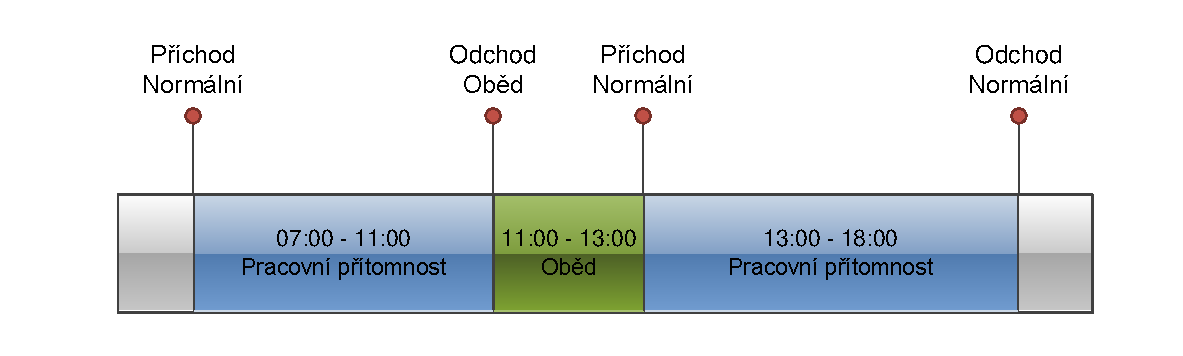
\includegraphics[scale=0.7]{visio/attnormal.pdf}
\caption{Časová osa běžného pracovního dne}
\label{fig:attn}
\end{figure}

Na obrázku \ref{fig:atts} je znázorněn pracovní den se služební cestou. Zaměstnanec nejprve zadá příchod do normální pracovní doby a s minutovým odstupem následuje služební odchod. Podobně musí zadat i návrat, nejprve zadá příchod do normální pracovní doby a s minutovým odstupem následuje normální odchod.
\begin{figure}[H]
  \centering
  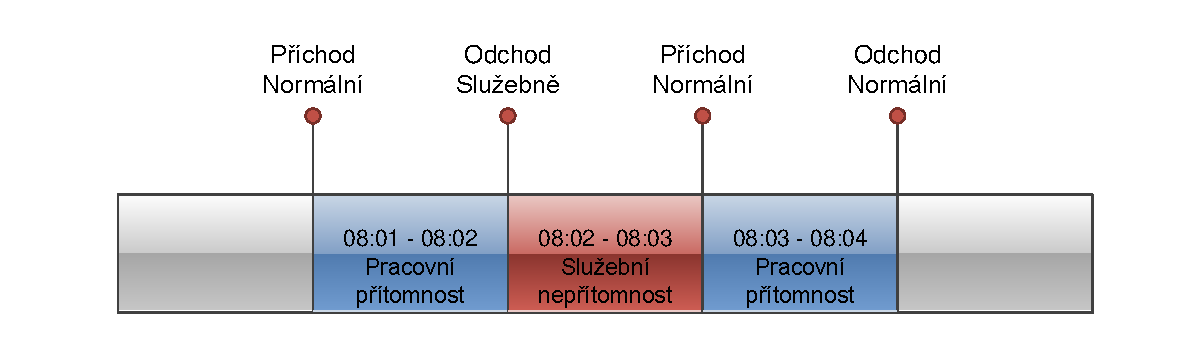
\includegraphics[scale=0.7]{visio/attservice.pdf}
\caption{Časová osa pracovního dne se služební cestou}
\label{fig:atts}
\end{figure}

\subsection{Vykazování odvedené práce}
Vykazování odvedené práce je jedním ze způsobů pro průběžnou kontrolu aktivit zaměstnanců. Ve firmě probíhá současně více projektů a bez výkazů by bylo velmi těžké sledovat průběžně náklady jednotlivých projektů. 
Díky evidenci je možné sledovat produktivitu jednotlivých zaměstnanců stejně jako nalézt slabá místa v pracovním procesu.
\\ \indent Výkazy práce jsou propojeny s docházkovým systémem a je možné porovnávat výstupy z těchto systémů. 

\subsection{Motivace}
Motivací pro vznik této práce bylo vytvořit mobilní aplikaci umožnující provádět každodenní agendu - zadávat příchody, odchody a výkazy práce pro zaměstnance, kteří často cestují a působí mimo sídlo organizace. Také snaha o využítí možností mobilního zařízení. Aplikace umožní pohodlné zadávání údajů a přinese možnost mít požadované informace po ruce.

Výsledná mobilní aplikace nemá nahradit vybrané části používaného systému, ale poskytnout efektivnější alternativu ve vybraných činnostech.


\section{Použitá technologie}
Současný systém je postaven na Oracle technologii. Jako uživatelské rozhraní používá Oracle Forms a data jsou ukládany v Oracle databázi.
 
\subsection{Oracle Forms}
Oracle Forms\cite{forms} je softwarový produkt vyvinutý společností Oracle. Slouží k vytváření formulářů, které interagují s Oracle databází. Jako programovací jazyk využívá PL/SQL. Produkt byl původně používán jako terminálové rozhraní pro komuikaci se serverem. Později byl přepracován do architektury klient-server.\\ \indent
Prostředí běhu zajišťuje defaultní správu transakcí. Díky tomu je Oracle Forms silný nástroj pro efektivní vývoj aplikací, jejichž primárním cílem je přístup k datům uložených v databázi. 

\subsection*{PL/SQL}
PL/SQL (Procedural Language/Structured Query Language) je procedurální nadstavba jazyka SQL od firmy Oracle založená na programovacím jazyku Ada.
\newpage
\subsection{Architektura}
Oracle Forms používá client-server architekturu. Klient funguje jako tlustý klient, který se kromě zobrazení dat stará o bussines logiku aplikace. Serverem je myšlel databázový server. Architektura je znázorněna na obr. \ref{fig:arch}

\begin{figure}[H]
  \centering
  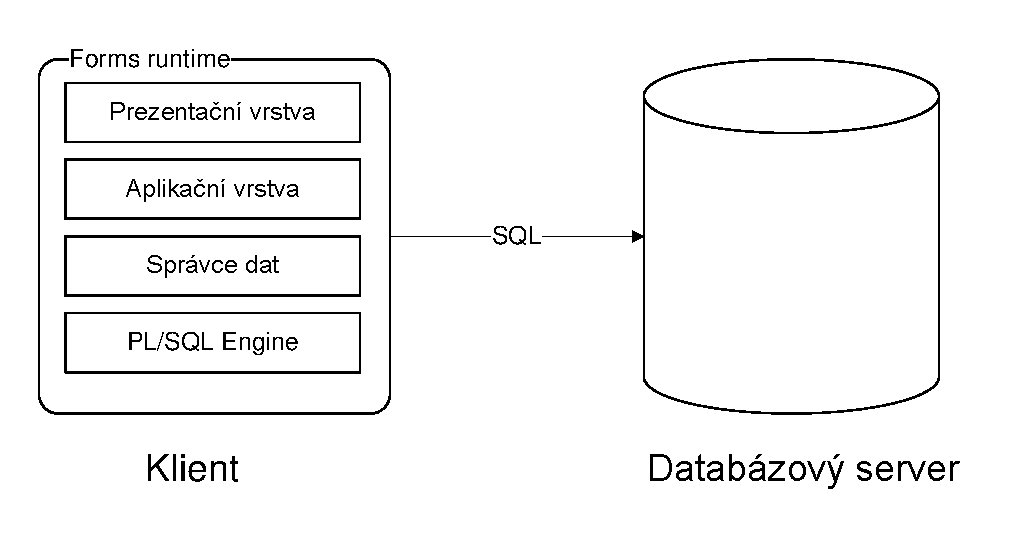
\includegraphics[scale=0.7]{visio/arch.pdf}
\caption{Klient-server architektura Oracle Forms aplikace}
\label{fig:arch}
\end{figure}
\paragraph{Forms prostředí běhu}
\begin{itemize}[noitemsep,nolistsep]
\item \textbf{Prezentační vrstva}\\
Zobrazuje informace pro uživatele formou grafického uživatelského rozhraní. Kontroluje zadávané vstupy.
\item \textbf{Aplikační vrstva}\\
Stará se o provedení aplikační logiky.
\item \textbf{Správce dat}\\
Stará se o zpracování dat se kterými formulář pracuje. Řídí databázové transakce.
\item \textbf{PL/SQL Engine}\\
Komponenta která zpracovává PL/SQL kód. Stará se o provedení procedurálního (PL) kódu a SQL kód předává ke zpracování databázi.
\end{itemize}

\paragraph{Databáze}
Databáze obsahuje data a kód, který s těmito daty pracuje (triggery, procedury, funkce). 

\newpage
\subsection{Komponenty formuláře}
\label{components}
Z hlediska architektury se Oracle Forms aplikace skládá z těchto celků:

\subsection*{Moduly}

\paragraph{Modul formuláře} 
Modul formuláře je hlavní komponenta aplikace. Poskytuje kód nezbytný pro interakci s úložištěm a uživatelským rozhraním. 
Data poskytovaná databází jsou reflektovaná v prvcích uživatelského rozhraní jako jsou textová pole, zaškrtávací políčka, přepínače, talčítka atd. Formulář je logicky organizován do bloků. Existují dva typy bloků: 
\begin{itemize}
\item Datový blok\\ Datový blok zobrazuje zdrojová data a poskytuje abstrakci pro způsob jakým jsou tato data získávána. Blok může být asociován s databázovou tabulkou, databázovým pohledem, uloženou procedurou, dotazem do databáze nebo transakčním triggerem. Asociace datového bloku a databázových dat standartně umožnujě přístup k těmto datům a jejich modifikaci.\\ \indent
Datové bloky mohou být navzájem svázany vztahem \emph{rodič - potomek}. Takový vztah představuje relaci 1:N databázových tabulek. Oracle Forms zajišťuje to, že při spojení mezi master a detail bloky se zobrazí pouze ty detail bloky, které jsou vázány na master blok přes cizí klíč. 

\item Řídící blok \\
Představuje blok, který nemá vztah k databázové tabulce. Řídící blok může obsahovat jakékoli prvky uživatelského rozhraní. Prvky mohou sloužit k uložení dočasných proměných nebo k zobrazení dat, které nemají přímou vazbu s databází. 
\end{itemize}

\paragraph{Modul menu} 
Modul obsahuje hiearchii menu. Každé menu obsahuje zvolitelné položky. Každý formulář obsahuje defaultní menu obsahující příkazy pro základní DML operace s databází CRUD.

\paragraph{Modul PL/SQL knihovny}
Modul obsahuje znovu využitelný kód, který může být využit jinými formuláři, menu či knihovnami. Programové jednotky knihovny mohou být funkce, procedury a balíčky. Programové jednotky jsou spouštěny na straně klienta. Mohou obsahovat business logiku. Knihovny jsou nezávislé na formuláři, jsou zaváděny dynamicky a mohou být zároveň využívány více formuláři.

\paragraph{Modul knihovny objektů}
Modul obsahuje znovu využitelné objekty. Řeší uskladnění, správu a distribuci těchto objektů, které mohou být využity jinými formuláři, menu či knihovnami. Využívání tohoto modulu přináší přínosy v podobě úspory paměti při běhu aplikace.

\begin{figure}[H]
  \centering
  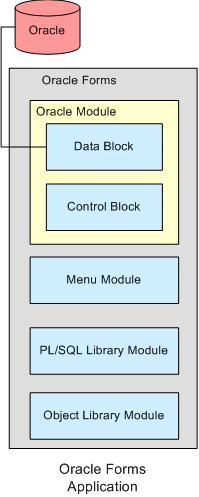
\includegraphics[scale=0.8]{obr/forms_arch3.png}
\caption{Komponenty Oracle Forms aplikace\cite{microsoft}}
\label{fig:arch3}
\end{figure}
\newpage
\subsection*{Triggery}
Aplikace v Oracle pracuje s následujícími typy triggerů:
\begin{itemize}
\item Block-processing triggers - jsou spouštěny při události na položce patřící tomuto bloku.
\item Interface event triggers - jsou spouštěny při události v uživatelském rozhraní formuláře.
\item Master-detail triggers - jsou spouštěny při události související se vztahem \emph{rodič - potomek} na daných blocích. Např. při změně položky rodiče příslušný trigger zobrazí příslušné položky v bloku potomka.
\item Message-handling triggers - zpracovávají zobrazení chybových či informačních zpráv.
\item Navigational triggers - jsou spouštěny při navigaci po položkách formuláře.
\item Query-time triggers - jsou spouštěny na úrovni bloku před a po dotazu do databáze.
\item Validation triggers - jsou spouštěny při validaci záznamu v položce.
\item Transactional triggers - vyvolají se při různých událostech související s interakcí s datovým úložištěm.
\end{itemize}
Pokud se jedná o datový blok, který je svázan s tabulkou v databázi, prostředí běhu automaticky zajištuje DML pro tyto bloky.
Pokud vývojář požaduje nestandartní akci při těchto úkonech, provede překrytí těchto triggerů s vlastní definovanou akcí.
\newpage
\subsection{Uživatelské rozhraní}
Při pohledu na uživatelské rozhraní se Oracle Forms aplikace skládá z těchto objektů:
\begin{figure}[H]
  \centering
  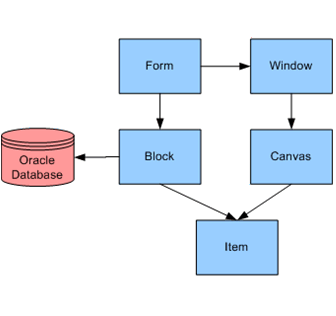
\includegraphics[scale=0.8]{obr/window.png}
\caption{Objekty uživatelského rozhraní Oracle Forms aplikace\cite{microsoft}}
\label{fig:gui}
\end{figure}


Plátno je objekt, na který je nakresleno celé GUI formuláře, tedy všechny viditelné objekty.  Okno ohraničuje plochu plátna, která bude zobrazena. Plátno je zobrazeno v okně. Blok sdružuje jednotlivé položky, které se vztahují ke stejnému databázovému objektu.
\subsection*{Seznam hodnot}
Seznam hodnot je prvek uživatelského rozhraní, který uživateli nabízí výběr hodnot. Výběr může být na základě pevně daných dat či dotazem do databáze.

\section{Důležité formuláře}
V této jsou popsány formuláře pro vybranou funčnost systému. 
 Konktrétně se jedná o formuláře pro zápis příchodů a odchodů na pracovistě a vykazování provedené práce.
\subsection{Zápis příchodů a odchodů}
\begin{figure}[H]
  \centering
  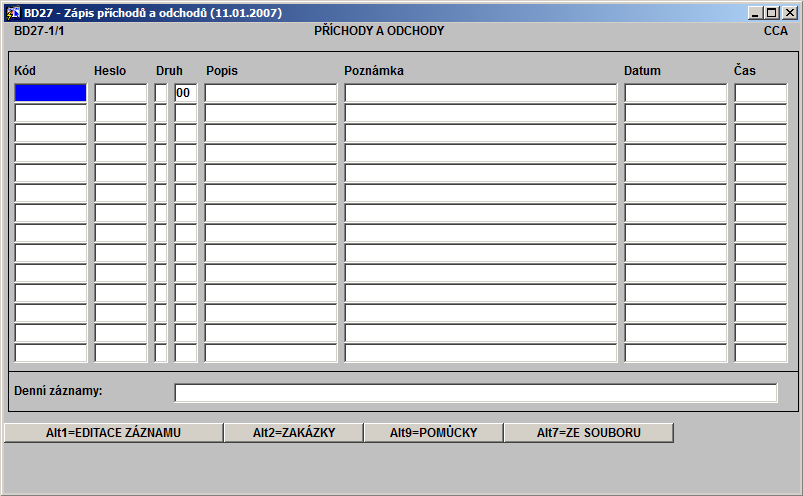
\includegraphics[scale=0.7]{obr/BD27.png}
\caption{Formulář pro zápis příchodů a odchodů}
\label{fig:att}
\end{figure}

\begin{itemize}[noitemsep,nolistsep]
\item Položky bloku pro zápis docházky
\begin{description}[noitemsep,nolistsep]
\item [Kód] - identifikátor zaměstnance.
\item [Heslo] - heslo zaměstnance. Pokud heslo nemá tak prázdné pole.
\item [Druh]  - druh události, příchod či odchod. Kód události.
\item [Popis] - doplní se automaticky podle kódu události.
\item [Poznámka] - volitelná poznámka.
\item [Datum] - datum události.
\item [Čas] - čas události.
\end{description}
\item Pole \emph{Denní záznamy} - zobrazuje denní docházku formou strukturovaného řetězce.
\item Pole s tlačítky - umožňuje akce, které nejsou pro potřeby cílové aplikace relevantní.
\end{itemize}

\newpage
\subsection{Výkaz práce}
\begin{figure}[H]
  \centering
  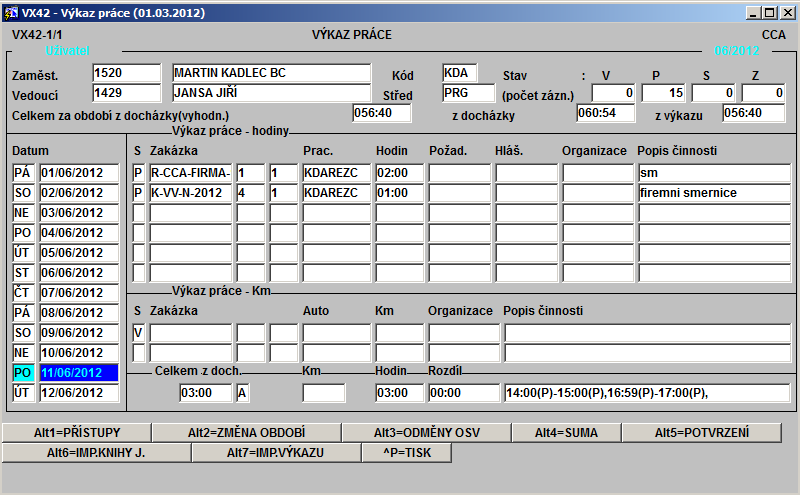
\includegraphics[scale=0.7]{obr/VX42.png}
\caption{Formulář pro pracovní výkazy}
\label{fig:rep}
\end{figure}

\begin{itemize}[noitemsep,nolistsep]
\item Položky bloku \emph{Uživatel} zobrazují identifikaci uživatele. Dále jsou zde statistiky stavů, ve kterých se nachází výkaz. V posledním řádku je zobrazen měsíční součet odpracovaného a vykázaného času.
\item V bloku \emph{Datum} je zobrazen měsíční kalendář.
\item V bloku \emph{Výkaz práce - hodiny} jsou výkazy pro zvolený den:
\begin{description}[noitemsep,nolistsep]
\item [Stav výkazu] - vypsaný, potvrzený, schválený, uzavřený.
\item [Zakázka] - identifikace zakázky.
\item [Pracoviště] - identifikace pracoviště.
\item [Hlášení] - chybové hlášení, které bylo podnětem pro tento úkol.
\item [Organizace] - identifikace organizace.
\item [Popis činnosti] - zaměstnancův popis odvedené činnosti.
\end{description}
\item V bloku \emph{Výkaz práce - Km} jsou výkazy jízd pro zvolený den:
\begin{description}[noitemsep,nolistsep]
\item [Auto] - identifikace vozidla.
\item [Km] - počet ujetých km.
\end{description}
\item Pole se statistikami zobrazuje denní součet odpracované doby, vykázané doby, ujetých km. 
\item Pole s tlačítky - jediná relevantní akce je změna zobrazovaného měsíce.
\end{itemize}

\chapter{Analýza}
V této kapitole se zabývám analýzou současného systému a návrhem cílové aplikace. Nejprve popíšu zvolenou architekturu a s tím související výběr typu webové služby. Dále popisuji datovou vrstvu jak současného systému tak i cílové aplikace a popisuju některé výhrady k datové vrstvě současného systému. Popisuji kde všude se nachází bussines logika relevantní pro funkčnost cílové aplikace a možnosti využití současného kódu. Popisuji způsob synchronizace dat mezi klientskou aplikací a podnikovou databází. Nakonec zmiňuji některé aspekty týkající se uživatelského rozhraní cílové aplikace.

\section{Architektura}
Při návrhu architektury jsem se rozhodoval mezi třemi variantami: přímé spojení Android aplikace ke vzdálené databázi pomocí JDBC, synchronizaci dat se vzdálenou databází pomocí Oracle Database Mobile Server a nakonec s využitím webové služby, která by sloužila jako rozhraní mezi klientskou aplikací a databázovým serverem.

\subsection{Přímé připojení k databázi}
Přestože příme připojení k Oracle databázi pomocí JDBC je možné, tuto variantu jsem zamítl. Připojení pomocí JDBC je primárně určeno pro stabilní síťové připojení, které má malou odezvu a nízkou ztrátu paketů. Využití JDBC by přineslo problémy v podobě špatné odezvy aplikace, kvůli znovu navazování spojení a vytváření nových databázových relací, které musely být v důsledku ztráty konektivity ukončeny.\\ \indent
Vzhledem k tomu, že původní Forms aplikace funguje jako tlustý klient, provádí veškerou bussines logiku. Tato logika je zapotřebí ke správné funkčnosti systému. Bylo by tedy nutné přenést tuto logiku na stranu klienta a potřeba komunikace se vzdálenou databází by byla větší než k pouhému přenesení dat.

\subsection{Oracle Database Mobile Server}
Oracle Database Mobile Server 11g\cite{mobile} je server zajišťující  synchronizaci dat mezi Oracle databází a mobilními zařízeními. Klíčovou vlastností tohoto produktu je synchronizační jádro, které je schopné zajistit synchronizaci velkého počtu mobilních zařízení se vzdáleným databázovým systémem. Přestože bylo toto synchronizační jádro navrženo pro stabilní připojení, je schopné zajistit spolehlivou funkci i při nestabilním připojení. V případě, že je spojení přerušeno synchronizace je pozastavena a po navázání spojení pokračuje v místě přerušení. Dále umožuje šifrování dat, jak pro přenos tak i pro jejich persistenci.\\ \indent
Tato varianta byla zamítnuta protože řeší pouze synchronizaci dat a neumožňuje zajistit provedení business logiky. Dalším důvodem je skutečnost, že její použití by vyžadovalo zakoupení licence pro tento server.\\ \indent
Server je možné spustit na serverech Oracle WebLogic Server a Oracle Glassfish. Mobilní klient, který běží na straně mobilního zařízení zajišťuje správu zařízení nutnou k synchronizaci. Tento klient je dostupný pro platfromy Java, Android, Blackberry, Windows a Linux.

\subsection{Webová služba}
Jako použitou architekturu jsem zvolil použití webové služby, která bude fungovat jako rozhraní mezi klientskou aplikací a databázovým serverem. Android klient v této architektuře funguje jako tenký klient spravující jen část funkčnosti z původního tlustého klienta. Business logika je umístěna na straně webové služby. Díky tomu že, webová služba bude umístěna v blízkosti firemní databáze, dojde k minimalizace odezev při zajištění business logiky systému. Mezi klientem a webovou službou se přenášejí pouzy data, která jsou opravdu nutná. \\ \indent
Z pohledu rozšiřitelnosti systému o další mobilní platformy se toto řešení jeví rovněž výhodně. Business logika by nebyla implementována ani na klientských aplikacích jiných platforem. Při změne logiky bude potřeba úpravy v kódu pouze na straně webové služby. Cílová architektura je vyobrazena na obrázku \ref{fig:deployment}.

\newpage
\subsection{Zvolená architektura}
Android aplikace funguje jako tenký klient, který se připojuje k webové službě. Webová služba přistupuje k samotné databázi. Jednotlivé komponenty jsou zobrazeny na obr. \ref{fig:deployment} a popsány níže:
\begin{itemize}
\item Android - aplikace je podporovaná od API 10. Obsahuje persistentní úložiště. Pro komunikace s webovou službou je určena \emph{AsyncTask} komponenta, která ukládá záznamy do databáze. Záznamy z databáze jsou zobrazeny v uživatelském rozhraní \emph{AsyncActvity}. Kromě tohoto scenáře se navíc bude úložiště automaticky synchronizovat s databázovým serverem prostřednictvím webové služby (není zobrazeno na obr. \ref{fig:deployment}).
\item Webová služba - je implementovaná v Java EE 6. Dodržuje RESTful principy s využitím Java API pro RESTful webové služby (JAX-RS) 1.1. Webová služba zpřístupňuje data pro klienta prostřednictvním \emph{Provider} komponent zpracovávající HTTP požadavek. Data jsou získávány z databáze pomocí \emph{DAO} (Data Access Object) objektů. Jako produkční aplikační server bude použit GlassFish 4.
\item Databázový server - hostuje databázi Oracle 10g, která obsahuje data ke kterým Android aplikace přistupuje. Navíc obsahuje databázové procedury a funkce, které jsou součástí bussines logiky používané v současném systému.
\end{itemize}
%Diagram zobrazující uvedené komponenty je na obr. \ref{obr:deployment}:
\begin{figure}[H]
  \centering
  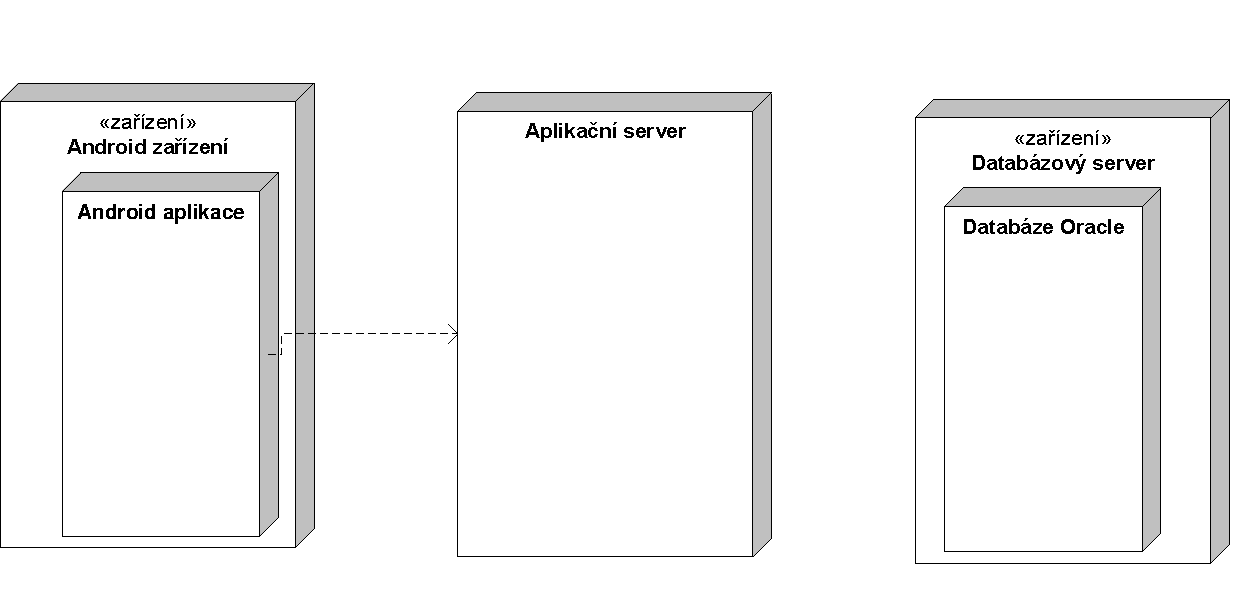
\includegraphics[scale=0.7]{visio/deployment.pdf}
\caption{Diagram nasazení}
\label{fig:deployment}
\end{figure}

\newpage
\section{Výběr typu webové služby}
Po zvolení architektury využívající webovou službu následuje výběr vhodného typu webové služby. V úvahu přichází varianty řešení s využitím SOAP protokolu či REST architektury.
\subsection{Representational State Transfer}
Representational State Transfer\cite{rest} (REST) je architektonický styl pro distribuovaný systém. Architektura využívá těchto vlastností:
\begin{description}
\item [Klient-server] Využívá se architektura klient-server z důvodu rozdělení zodpovědností pro komponenty systému (\emph{Separation of concerns}). Klient je zodpovědný za uživatelské rozhraní, díky tomu je získána větší přenositelnost na jiné platformy. Na straně serveru, který je zodpovědný za datovou vrstvu, se získá výhoda větší škálovatelnosti. 
\item [Bezestavost] Komunikace probíhá bezestavově. Každý požadavek musí obsahovat všechny informace nutné k jeho vyřízení. Pokud je nutné pamatovat si stav, je to zodpovědností klienta. Díky tomu se zvyšuje spolehlivost systému, protože to usnadňuje zotavení se ze stavu částečného selhání. Také se zvyšuje škálovatelnost, protože server si nemusí udržovat informaci o stavu a díky tomu potřebuje méně zdrojů. Rovněž je snažší takový server implementovat.
\item [Mezipaměť] Data přijímaná jako odpověď ze serveru musí být označena, zda mohou být uložena do mezipaměti klienta či nikoli. Pokud jsou uložena, klient je může využít opakovaně. Díky tomu je snížen počet interakcí. 
\item [Jednotné rozhraní] Zdroje jsou identifikovány pomocí URI, které ale nezávisí na tom jakým způsobem budou data vrácena klientovi. Každý požadavek na server obsahuje informaci jakým způsobem mají být data zpracována (pomocí MIME hlavičky HTTP požadavku).  
\item [Vícevrstevný systém] Klient nemusí získávat data přímo ze serveru na který se obrací. Server může fungovat jako prostředník, který je sám v roli klienta vůči jinému uzlu systému. Rozdělení systému do více vrstev může být využito k zapouzdření zastaralých služeb, k ochraně nových služeb před zastaralými klienty či zjednodušení kompoment díky sdílení zřídka využívaných služeb. Jiným přínosem může být zlepšení škálovatelnosti díky rozložení zátěže mezi více uzlů na stejné vrstvě systému.
\item [Kód na požádání] Server může klientovi poskytovat kód, který je spustitelný na straně klienta a přinést tak další funkcionalitu.
\end{description}

\subsubsection*{RESTful web API}
Systém který využívá principy REST se označuje jako \emph{RESTful}. RESTful webové API je webové API využívající HTTP a REST principy. Jedná se o kolekci zdrojů s těmito definovanými aspekty: 
\begin{itemize}
\item základní URI pro webové API
\item typ internetového média dat poskytovaných API (JSON, XML nebo jiný splňující hypertextové standarty)
\item množina operací podporovaná webovým API pomocí HTTP method
\begin{itemize}
\item k získání zdroje se používá GET metoda
\item k aktualizaci zdroje se používá PUT metoda
\item k vytvoření zdroje se používá POST metoda
\item ke smazání zdroje se používá DELETE metoda
\end{itemize}
\item API musí být řízeno hypertextově
\end{itemize}

\subsection{Simple Object Access Protocol}
Simple Object Access Protocol (SOAP) je standardizovaný protokol pro výměnu dat mezi webovými službami. Protokol řídí výměnu zpráv mezi poskytovatelem a konzumentem služby. Komunikace probíhá většinou pomocí HTTP protokolu, který je použit z důvodu lepší prostupnosti přes zabezpečující síťové prvky.\\ \indent
Existuje několik různých druhů šablon pro komunikaci na protokolu SOAP. Nejznámější z nich je RPC šablona, kde jeden z účastníků komunikace funguje jako klient a druhý jako server. Server odpovídá na požadavky klienta.\\ \indent
Na obr. \ref{fig:soap} je znázorněn vztah základních technologií používaných u webové služby využívající SOAP protokol.
\begin{figure}[H]
  \centering
  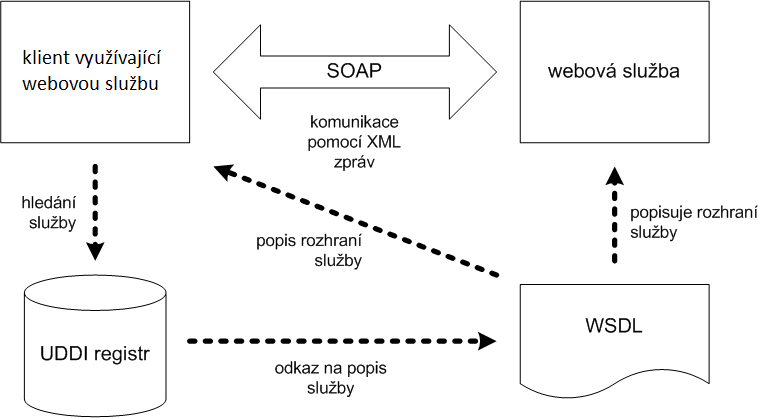
\includegraphics[scale=0.8]{obr/komunikace-webservices.png}
\caption{Vztah tří základních technologií (SOAP, WSDL a UDDI) webových služeb\cite{websluzby}}
\label{fig:soap}
\end{figure}

\begin{description}
\item [Webová služba] Poskytovatel služby. Ke službě se přistupuje pomocí \emph{endpoint} URL. \emph{Endpoint} URL definuje umístění služby, kde poskytovatel očekává příchozí požadavky.
\item [Klient] Konzument služby, který si v UDDI registru vyhledá požadovanou službu. Poté sestaví zprávu podle specifikace a kontaktuje poskytovatele.
\item [UDDI\cite{uddi}] (Universal Description, Discovery, and Integration) registr je místo, které poskytuje informace o dostupných službách a jejich poskytovatelích. 
\item [WSDL\cite{wsdl}] (Web Services Description Language) je jazyk, kterým je popisována funkcionalita poskytovaná webovou službou. WSDL soubor poskytuje strojově čitelný popis toho, jak může být služba volána, jaké parametry očekává a jaké datové struktury vrací.
\end{description}

\subsection{Odůvodnění výběru}
Vzhledem k tomu, že webová služba má sloužit ke správě vzdálené databáze, jeví se REST se svojí CRUD maticí operací jako jasná volba. Při použití REST společně s přenosem dat ve formátu JSON bude objem přenesených dat malý, což je důležité, protože klientskou aplikací má být mobilní zařízení. Webovou službu využívající REST bude ve srovnání se SOAP snadnější implementovat. Jedinou nevýhodou bude bezestavovost komunikace, která přináší nutnost provádění procesu autentizace pro každý požadavek.

\section{Datová vrstva}
V této kapitole analyzuji datovou vrstvu systému. Identifikuji datové entity, které jsou relevantní pro zkoumanou část systému a popisuji některé nedostatky používaného datového schématu.

\subsection{Datový model}
V následujícím diagramu (obr. \ref{fig:object}) zobrazuji entity nacházející se v systému, které jsou relevantní pro zkoumanou část systému. Další tabulky a číselníky jsou pro jednoduchost vypuštěny.
\begin{figure}[H]
  \centering
  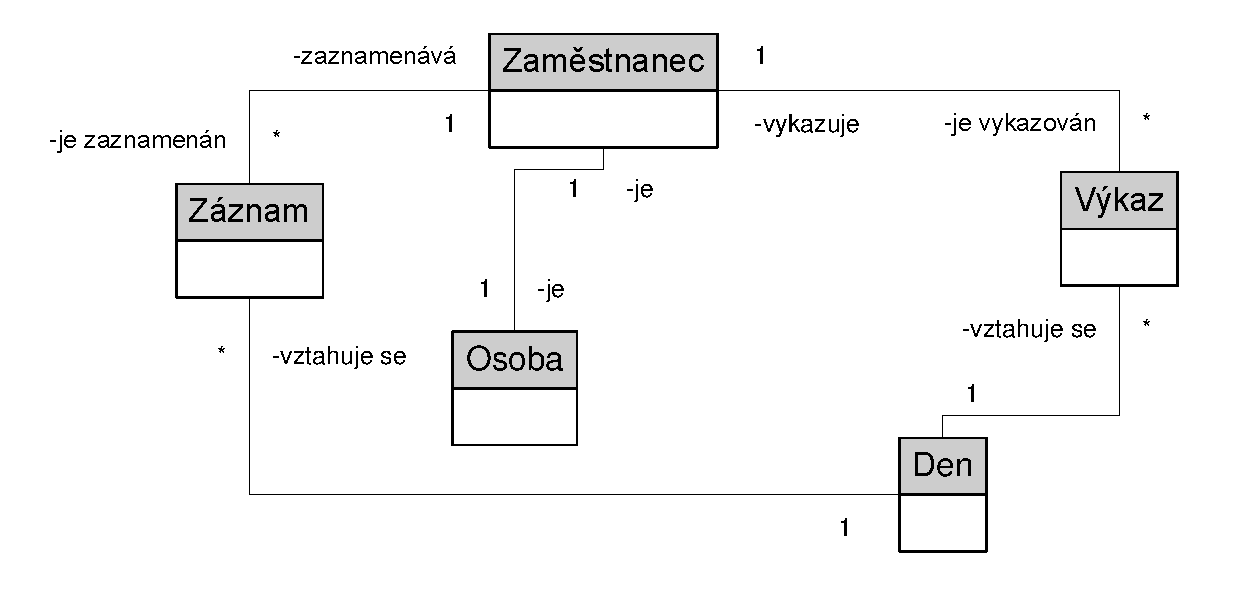
\includegraphics[scale=0.6]{visio/object.pdf}
\caption{Diagram relevantních entit nacházejících se v systému}
\label{fig:object}
\end{figure}
\noindent
Jednotlivé entity a jejich popis:

\begin{description}
\item [Záznam]
Příchod nebo odchod na pracoviště. Obsahuje informaci o čase, datu, účelu a případně zaměstnancův krátky popis události.
\item [Výkaz]
Pracovní výkaz. Obsahuje informaci o čase, datu, osobě zadavatele, osobě řešitele, vykazované době, vazbu na zakázku či chybové hlášení, stav výkazu, zaměsnancův popis činnosti.
\item [Zaměstnanec]
Zaměstnanec a jeho příslušnost k pracovnímu oddělení, funkce, vedoucí pracovník a typ úvazku. 
\item [Osoba]
Podrobnější informace o osobě zaměstnance, jméno, pracovní zkratka.
\item [Den]
Den ke kterému se váže výkaz či záznam. Slouží k rozlišení pracovních dnů a svátků.
\end{description}

\subsection{Datový model v mobilní aplikaci}
Na straně Android aplikace budou persistentně ukládány pouze tyto entity:

\begin{description}
\item [Záznam]
Příchod nebo odchod na pracoviště pro uživatele, který rovněž vytváří záznamy prostřednictvím mobilní aplikace. Dále záznamy ostatních uživatelů, které si uživatel stáhne k prohlížení.
\item [Výkaz]
Výkazy práce které si uživatel stáhne k prohlížení.
\item [Zaměstnanec] 
Lokální databáze zaměstnanců, kde se ukládají základní údaje společně s informací o poslední docházkové události. Databáze zaměstnaců bude sloužit pro naplnění rozbalovací nabídky pro výběr zaměstnance, která bude součástí uživatelského rozhraní.
Další využití je pro zobrazení seznamu přítomných zaměstnanců.
\end{description}

Data budou ukládané ve třech tabulkách SQLite databáze. Datový model nebude řešit referenční integritu těchto tabulek. Zajištění referenčí integrity je záležitostí databáze systému a její zajištění na straně klienta je zbytečné.

\newpage
\subsection{Práce s datumem a časem}
Při návrhu datového modelu jsem řešil problém pomocí jakého datového typu vyjadřovat údaj o čase či datu. V Oracle databázi je použit datový typ Date. SQLite databáze nabízí tři způsoby jako ukládat informaci o čase:
\begin{itemize}
\item \textbf{TEXT} podle ISO8601 normy ve formátu "YYYY-MM-DD HH:MM:SS.SSS".
\item \textbf{REAL} podle Juliánského kalendáře, počet dní od poledne 24. Listopadu roku 4714 před kristem (Greenwichského času).
\item \textbf{INTEGER} jako Unix Time, počet sekund 1970-01-01 00:00:00 UTC.
\end{itemize}

\noindent
Pro uložení v SQLite databázi jsem zvolil typ INTEGER. V aplikaci (Android klient, webová služba) jsem se rozhodl reprezentovat časový údaj pomocí primitivního typu long. Měl jsem k tomu řadu dobrých důvodů:
\begin{itemize}
\item odpadá starost s formátem datumu při serializaci a deserializace JSON řetězce
\item snadné porovnávání hodnot pomocí relačních operátorů
\item sníží se počet konverzí v aplikaci (např. pro výpočet pozice pro vykreslení komponenty v UI)
\end{itemize}

Také jsem se ujistil, že rozsah typu long je pro potřeby aplikace dostačující. Srovnání použitých datových typů je znázorněno v tabulce \ref{tab:cas}. 

\begin{table}[H]
\centering
\begin{tabular}{| p{2.5cm} | c | c | c |}
\hline
Datový typ &  Minimální hodnota & Maximální hodnota & Přesnost \\ \hline
Oracle Date &   January 1, 4712 BCE  &  December 31, 4712 CE &  s \\ \hline
\parbox[c][1cm][c]{5cm}{SQLite\\ INTEGER} &  2.12.292269055 BC  & 17.8.292278994 AD &  ms \\ \hline
Java long & 2.12.292269055 BC   & 17.8.292278994 AD &  ms \\ \hline
\end{tabular}
\caption{Datové typy reprezentující časový údaj}
\label{tab:cas}
\end{table}
%\parbox[pos][height][inner-pos]{width}{text}

\newpage
\subsection{Výhrady k datové vrstvě}
Při práci s datovou vrstvou aplikace jsem vyhodnotil některé vlastnosti jako důsledek špatného návrhu datového schématu.
\subsubsection*{Tabulka bez primárního klíče}
Tabulka pro evidenci docházkových události neobsahuje primární klíč. To je velký problém, protože klient měnící data potřebuje jednoznačně identifikovat záznam. Absenci primárního klíče lze vyřešit indetifikací záznamu pomocí pseudosloupce ROWID. Hodnota ROWID se skládá z těchto hodnot:
\begin{itemize}[noitemsep,nolistsep]
\item číslo datového objektu 
\item číslo datového bloku v souboru, kde se záznam nachází
\item pozice řádku v datovém bloku 
\item číslo datového souboru, kde se záznam nachází. Číslo souboru je relativní vzhledem k tabulkovému prostoru.
\end{itemize}
Pomocí ROWID lze tedy jednoznačně identifikovat záznam. Bohužel kvůli k tomu, že jeho hodnota je relativní vzhledem k tabulkovému prostoru, tak jeho použití jako unikátního identifikátoru může selhat v těchto situacích:
\begin{itemize}[noitemsep,nolistsep]
\item záznam je fyzicky přemístěn do jiného tabulkového prostoru či jiné databáze, v tom případě bude vygenerován nový ROWID a záznam uložený na klientovi bude odkazovat na neexistující umístění či v horším případě na existující ale jiný záznam
\item pokud uživatel smaže záznam prostřednictvím jiného klienta zatímco má záznam uložený na svém mobilním zařízení, může rovněž dojít k situaci, kdy záznam uložený na klientovi bude odkazovat na neexistující umístění nebo na existující ale jiný záznam 
\end{itemize}

Vhodným řešením by byla změna databázového schématu tabulky pro záznam docházkových událostí a to přidáním primárního klíče. Vzhledem k tomu že se se záznamy pro docházku po zpracování aktuální měsíce již dále nepracuje, tak případná změna starších dat nemůže napáchat reálné škody. 
\subsubsection*{Schéma pro docházku}
Záznam o příchodu či odchodu reprezentuje vždy jeden záznam pro každou z těchto událostí. Při práci s těmito daty na aplikační vrstvě je nutné vždy spárovat příchody a odchody týkající se daného zaměstnance. Je na zvážení zda nemohlo být datové schéma navržené lépe např. příchod či odchod by představoval jeden záznam v tabulce nebo pokud by každý odchod odkazoval na příslušný příchod. Kromě jednoduššího zpracování na aplikační vrstvě by byla rovněž snažší kontrola chybného vstupu, kdy zaměstnanec omylem zadá dva příchody či odchody následující po sobě. Taková kontrola se v současnosti v systému neprovádí.

\subsubsection*{Datum a čas odděleně}
Datum a čas docházkové události se uchovává odděleně, kdy každá z těchto hodnot má svůj příslušný sloupec. Je na zvážení, zda tyto údaje neměly být ukládány jako jedna hodnota.

\subsubsection*{Čas jako reálné číslo}
Jako špatné rozhodnutí hodnotím skutečnost, že údaj o čase je reprezentován jako reálné číslo nabývající hodnot <0.0, 24.0>.  Tento fakt přináší komplikace při převodu čísla na hodiny a minuty. Údaj o čase by mohl být reprezentován jako celé číslo představující minuty.

\section{Business logika}
Při analýze zdrojového kódu zkoumané části současného systému jsem indetifikoval kód v těchto umístěních:
\vspace{-2mm}
\begin{itemize}%[noitemsep,nolistsep]
\item triggery, které jsou součástí vybraných formulářů
\item knihovny využívané vybranými formuláři
\item databázové triggery, funkce a procedury
\end{itemize}
Veškerý kód je napsán v jazyce PL/SQL.
\subsection{Triggery formuláře}
Z množiny triggerů (zmíněných v \ref{components}) použitých ve formulářích bude nutné implementovat triggery pracující na datovém bloku a validační triggery. Ostatní typy triggerů nemají v kontextu implementované aplikace smysl. Konkrétně se jedná o tyto:

%Block-processing triggers Validation triggers
\begin{description}
\item [Block-processing triggery:] On-Delete, On-Insert, On-Update, Pre-Delete, Pre-Insert, Pre-Update
\item [Validation triggery:] When-Validate-Item
\end{description}

\subsection{Databázové triggery}
Databázové triggery se provádějí při definovaných událostech jako vložení, změna či smazání záznamu do konkrétní tabulky. Jejich činnost provádí databáze a to bez ohledu na to, který klient k databázi přistupuje. Jejich funkčnost tedy zůstává nezměněna při použití společně s webovou službou.

\subsection{Databázové uložené funkce a  procedury}
Funkce a procedury uložené v Oracle databázi lze volat z aplikace prostředky jazyka Java. Slouží k tomu rozhraní \emph{java.sql.CallableStatement}. Ukázka volání uložené funkce z Javy:\\

\begin{lstlisting}
CallableStatement callableStatement = conn.prepareCall(
"{? = call IMISOID_HESLO_WRAPPER(?, ?)}");
callableStatement.setString(2, icp);
callableStatement.setString(3, heslo);
callableStatement.registerOutParameter(1, OracleTypes.NUMBER);
callableStatement.executeUpdate();
BigDecimal bool = callableStatement.getBigDecimal(1);
\end{lstlisting}

\subsubsection{Funkce vracející typ BOOLEAN}
Problém nastává pokud uložená funkce vrací typ BOOLEAN. Ovladač databáze Oracle JDBC nepodporuje typ BOOLEAN jako návratový datový typ \cite{limitation}. Řešením je použití obalující procedury, která zpracuje výsledek volané procedury vracející BOOLEAN, ale sama vrací podporovaný datový typ (např. NUMBER). Ukázka takové obalující procedury: \\

\begin{lstlisting}
FUNCTION IMISOID_HESLO_WRAPPER(PIcp in Varchar2, PHeslo in Varchar2) RETURN NUMBER AS
  myvar boolean;
BEGIN
  myvar := ccap_heslo_pkg.SpravneHeslo(PIcp,PHeslo);
  
  IF myvar THEN
    RETURN 1;
  ELSE
   RETURN 0;
  END IF;  
 
END;
\end{lstlisting}

\subsection{Forms knihovny}
Další zdrojový kód používáný formuláři se nachází v knihovnách. Ačkoli se jedná o nezávislé jednotky, není způsob jak použít procedury v nich obsažené z prostředí jazyka Java.

\subsection{Shrnutí}
Část současného kódu zajišťující business logiku formulářů bude muset být přepsána do jazyka Java. Tento přepsaný kód bude umístěn do webové služby. Konkrétně se jedná o zdrojový kód umístěný v současných formulářích a knihovnách, které jsou jimy používány. Kód umístěný na straně databáze lze využít a nebude muset být přepsán.

\newpage
\section{Synchronizace dat}
V současném systému uživatel zadává data prostřednictvím příslušného formuláře. Změny jsou aplikovány bezprostředně po uložení během databázové transakce. Mobilní klient přináší nový způsob použití - data lze zadat i v režimu offline, kdy mobilní klient není v dosahu webové služby. Tyto data jsou uložena persistentně na straně klienta a jsou synchronizována až ve chvíli kdy je možná komunikace s webovou službou.\\ \indent
Synchronizace se týká pouze dat pro docházku uživatele. Ostatní data jsou prostřednictvím mobilního klienta pouze zobrazována. Je třeba počítat s tím, že záznamy přidané na straně klienta v režimu offline nemusí být přijaty při synchronizaci z důvodu porušení business pravidel a uživatel by měl být o této skutečnosti vhodně informován.

\subsection{Obousměrná synchronizace}
Při obousměrné synchronizaci se odesílají data ze strany klienta na server tak i opačným směrem ze serveru na klienta. Klienta lze navrhnout tak, aby si uchovával informaci o změnách na svojí straně. Při analýze databázového schématu pro docházku v současném systému jsem zjistil, že databáze neuchovává informaci o změnách na svojí straně. Beze změny této skutečnosti není možné sledovat změny na straně databáze. Výsledkem je poněkud neefektivní způsob synchronizace, kdy klient odesílá na server pouze změny, zatímco ze serveru stahuje všechna data pro daného uživatele a období.
\\ \indent
Celkový průběh synchronizace je znázorněn v diagramu \ref{fig:sync}. Klient nejprve odešle všechny svoje změny na server. Poté smaže všechny úspěšně odeslaná data. Bez smazání by nebylo možné zjistit, že na serveru došlo ke změně či smazání dat jiným klientem. Poté už zbývá pouze stažení aktuálních dat ze serveru. Data která na klientovi nebyla smazána z důvodu neúspěsného odeslání na server, zůstávají do té doby, než uživatel tyto data upraví tak aby vyhovovali bussines pravidlům. Dalším důvodem pro neúspěšnou synchronizaci může být přerušení spojení. Data zůstavají na klientovi, až do doby úspěšného pokusu o synchronizaci.
\begin{figure}[H]
  \centering
  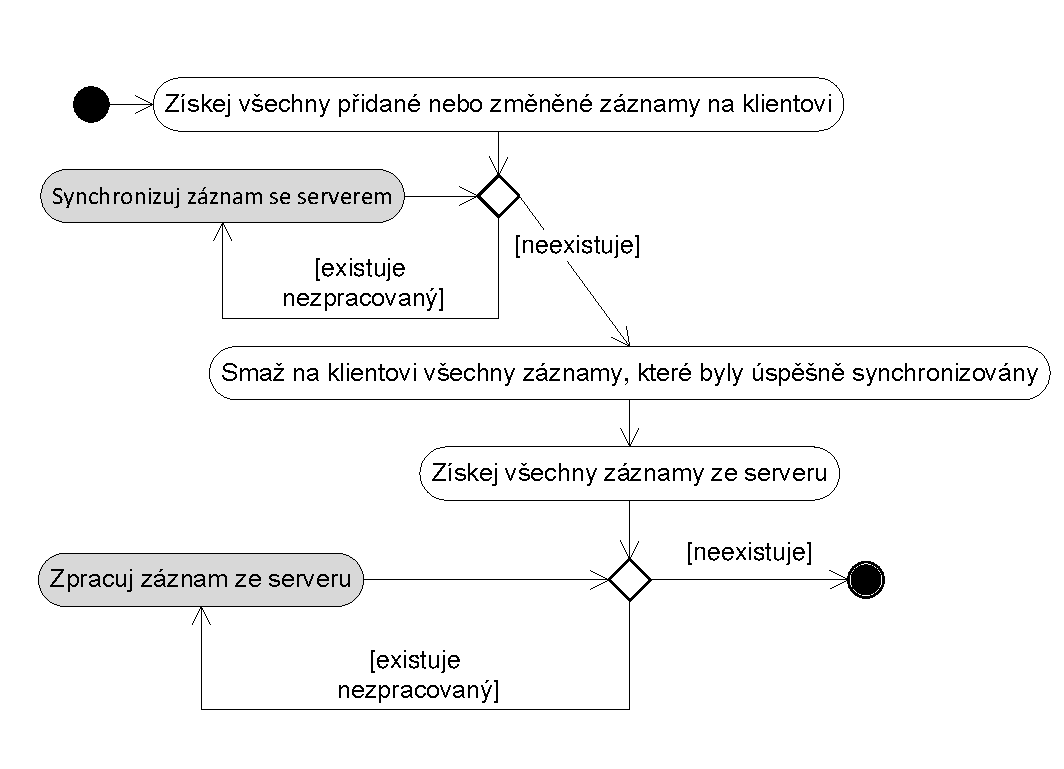
\includegraphics[scale=0.7]{visio/sync.pdf}
\caption{Diagram aktivit pro průběh synchronizace}
\label{fig:sync}
\end{figure}

Diagram \ref{fig:syncup} podrobněji rozepisuje průběh odeslání požadavku na server. Pokud klient nemá server ID záznamu, znamená to, že záznam byl vytvořen na straně klienta a odesílá se požadavek na vytvoření. Pokud klient zná server ID může požadovat smazání nebo aktualizaci záznamu. 

Diagram \ref{fig:syncdown} podrobněji rozepisuje průběh přijetí záznamu ze serveru.
\begin{figure}[H]
  \centering
  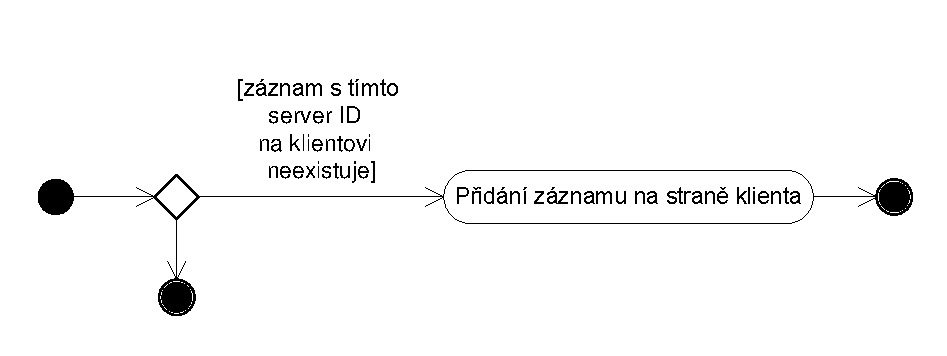
\includegraphics[scale=0.7]{visio/syncdown.pdf}
\caption{Diagram aktivit pro přijetí záznamu ze serveru}
\label{fig:syncdown}
\end{figure}

\begin{figure}[H]
  \centering
  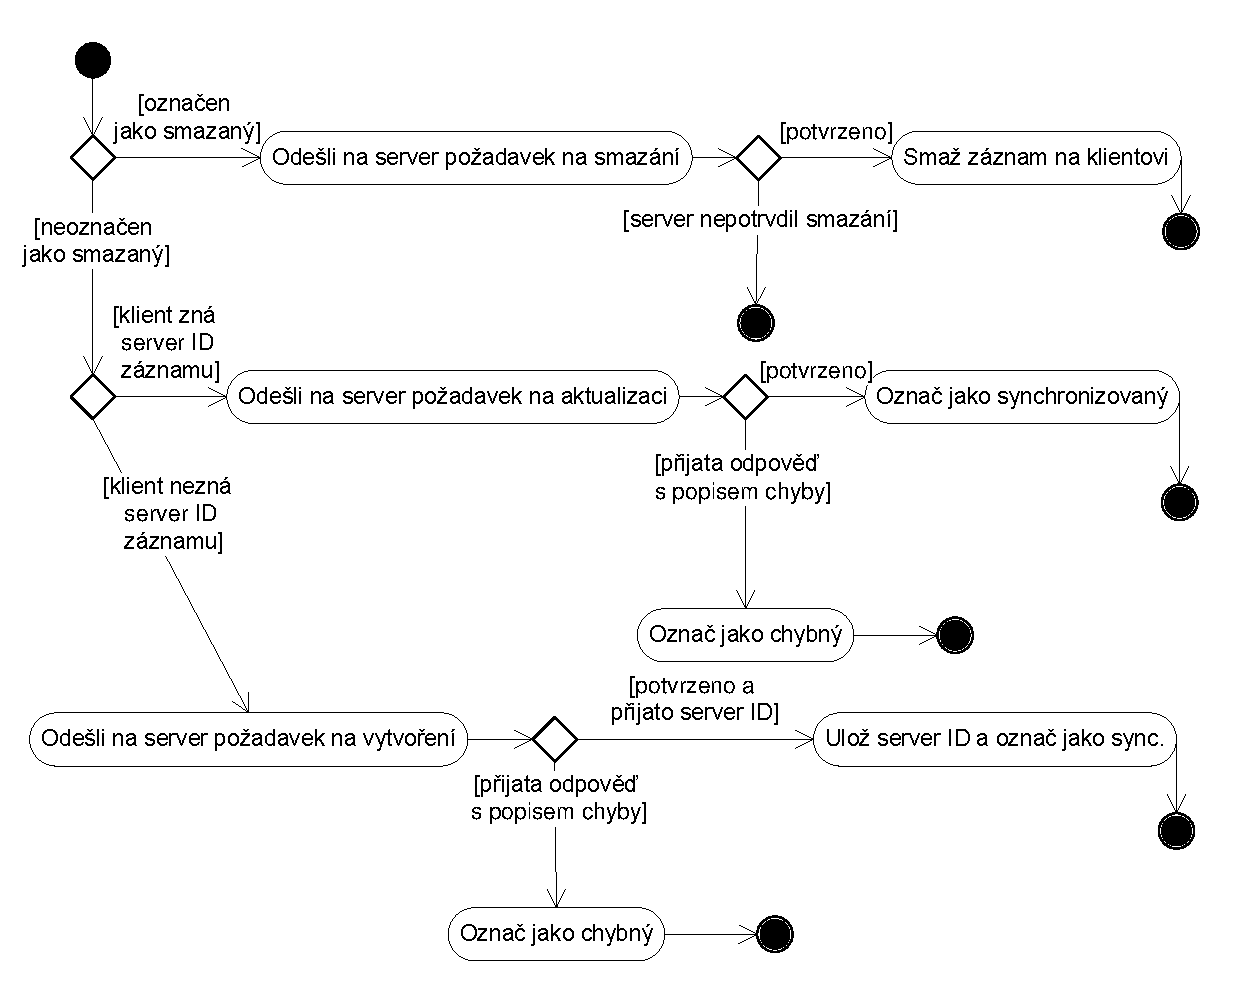
\includegraphics[scale=0.7]{visio/syncup.pdf}
\caption{Diagram aktivit pro odeslání požadavku na server}
\label{obr:syncup}
\end{figure}
\vspace{-8mm}
\subsection{Obousměrná synchronizace s úpravou databáze}
Jiná varianta řešení problému synchronizace dat, která se snaží eliminovat nedostatky předchozí varianty, by vyžadovala změny v databázovém schématu současného systému. U každého záznamu by byla přidána informace o poslední změně záznamu s vhodnou časovou přesností. Pokud by došlo k požadavku na smazání záznamu, nebyl by záznam skutečně smazán, ale pouze nastaven přížnak smazaného záznamu. Při použití tohoto řešení by bylo možné synchronizovat oběma směry pouze změny ze strany klienta i serveru. \\ \indent
Klient který iniciuje synchronizaci nejprve odešle na server požadavek ke kterému připojí údaj o času provedení poslední synchronizace. Server odesílá ke klientovi pouze ty data, která se změnila po tomto termínu. Poté klient odesílá svoje změny na server.

\subsection{Řešení kolizí}
Kolize teoreticky nastane vždy, když se v době od poslední synchronizace změní stejná data jak na serveru, tak v zařízení. Vzhledem k tomu, že server neukládá informaci o čase poslední synchronizace a není tedy možné zjistit že vůbec došlo ke změne dat, tak mobilní klient vždy přepíše záznam na serveru.

\subsection{Srovnání}
V obou případech řešení je iniciátorem synchronizace klient. Druhá varianta by oproti první přinesla úsporu množství přenesených dat. Vzhledem k tomu, že druhá varianta by vyžadovala změnu v databázovém schématu současného systému, zvolil jsem první variantu i přesto, že z hlediska efektivity synchronizace je to horší řešení.

\section{Uživatelské rozhraní}
Uživatelské rozhraní současného systému je desktopové rozhraní. Při implementaci mobilního klienta budou muset být respektovány vlastnosti takového zařízení jako je velikost displeje či nepohodlnost používání softwarové klávesnice.\\
\indent Uživatel mobilního zařízení nebude muset zadávat veškeré vstupy jako na formuláři \ref{fig:att}, protože zařízení si bude pamatovat jeho indentitu. Dále bude vhodné využít některé komponety poskytované Android SDK jako je např. widget pro kalendář.

\chapter{Zabezpečení}
V následující kapitole se zabývám zabezpečením aplikace. Popisuji několik možných variant z hlediska ověřování identity uživatele. Na závěr vysvětluji výběr zvoleného řešení.
\section{Autentizace a autorizace}
Při analýze současného systému jsem zjistil, že informace o docházce a výkazech zaměstnanců jsou dostupné všem ostatním uživatelům (údaje týkající se nadřízených pracovníků jsou dostupné i podřízením). Dalším zajímavostí je, že heslo používané k zadání docházky je pro uživatele nepovinné (má ho jen ten uživatel, který si ho nastavil). 

\subsection*{Autentizace}
Autentizace je proces ověření proklamované identity subjektu. Uživatel se identifikuje pomocí svého uživatelského jména a hesla.

\subsection*{Autorizace}
Autorizace je proces získávání souhlasu s provedením nějaké operace. Uživatel musí zadávat svoj přístupové údaje při zadání každého záznamu docházky. 

\subsection*{Riziko poškození systému}
Webová služba umožňuje čtení a úpravu docházkových dat a dále čtení dat o výkazech práce a zaměstnancích. Dále používá některé databázové objekty jako jsou procedury a funkce, které pracují s těmito daty. Je vhodné aby aplikace měla přístup pouze k těm databázovým objektům, které jsou relevantní pro navrženou funkčnost aplikace. To je vhodné pro maximální zabezpečení okolního systému a minimalizaci případných rizik při zneužití či chybě v aplikaci. Toto je zodpovědností databázového administrátora organizace a v této práci se touto problematikou dále nezabývám.

\subsection*{HTTP Basic autentizace}
Klient posílá autentizační hlavičku jako součást HTTP požadavku na server. Jméno a heslo je zasláno jako jeden textový řetězec oddělený dvojtečkou. Výsledný řetězec je poté zakódován metodou Base64. Uživatelské jméno a heslo se tedy posílá v zakódované podobě. Nejedná se ale o kryptografické zabezpečení přihlašovacích údajů. Použití této metody předpokládá použití zabezpečeného komunikačního kanálu mezi klientem a serverem.


\section{VPN pro vzdálený přístup}
Virtuální privátní síť  je prostředek pro propojení počítačů v prostředí nedůvěryhodné sítě. Díky VPN spojení mohou počítače komunikovat tak, jako by byly součástí důvěryhodné sítě.

\subsection*{Vlastnosti připojení VPN}
\begin{itemize}[noitemsep,nolistsep]
\item Zapouzdření\\ Při použití technologie VPN jsou data zapouzdřena pomocí hlavičky obsahující směrovací informace, které umožňují průchod dat přes tranzitní síť.
\item Ověřování\\
Klient a VPN server se vzájemně ověřují na úrovni počítače. Android má integrovanou podporu pro VPN využívající protokoly PPTP, L2TP a IPSec.
\item Šifrování dat\\
Pro utajení dat během jejich přenosu sdílenou nebo veřejnou tranzitní sítí jsou data na straně odesílatele zašifrována a na straně příjemce dešifrována. Šifrování a dešifrování je založeno na tom, že odesílatel i příjemce používají společný šifrovací klíč.
\end{itemize}

Webová služba je tedy umístěna na serveru uvnitř firemní sítě. Pokud klient chce komunikovat s webovou službou musí tak činit 
prostřednictvím sítě VPN.

\section{Autentizace proti databázi}
Klient i server jsou součástí jedné VPN sítě, která zajišťuje důvěryhodný komunikační kanál.  Klient posílá na server HTTP požadavek jehož součástí je autentizační hlavička nesoucí uživatelské jméno a heslo. Webová služba ověří jméno a heslo pomocí databázové procedury. Jméno a heslo uživatele je uloženo v databázi. Implementované řešení je znázorněno na obr. \ref{fig:auth} který zobrazuje sekveční UML diagram v případě úspěšné autentizace.
\begin{figure}[H]
  \centering
  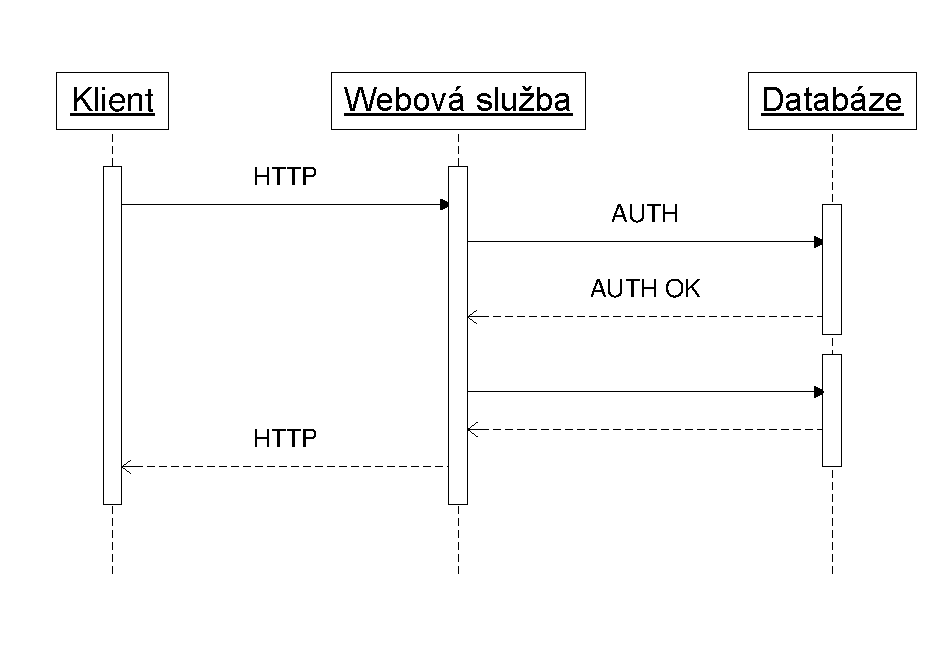
\includegraphics[scale=0.8]{visio/auth.pdf}
\caption{Diagram aktivit při úspěšné autentizaci}
\label{fig:auth}
\end{figure}

\section{Autentizace proti LDAP}
Alternativním řešením by bylo ověřování uživatelů pomocí LDAP adresáře. Organizace již LDAP používá v některých dalších firemních systémech. Toto řešení se liší v tom, že dotaz na ověření identity uživatele probíhá k LDAP adresáři a nikoli k databázi. Implementované řešení je znázorněno na obr. \ref{fig:authldap}, který zobrazuje sekveční UML diagram v případě úspěšné autentizace.
\begin{figure}[H]
  \centering
  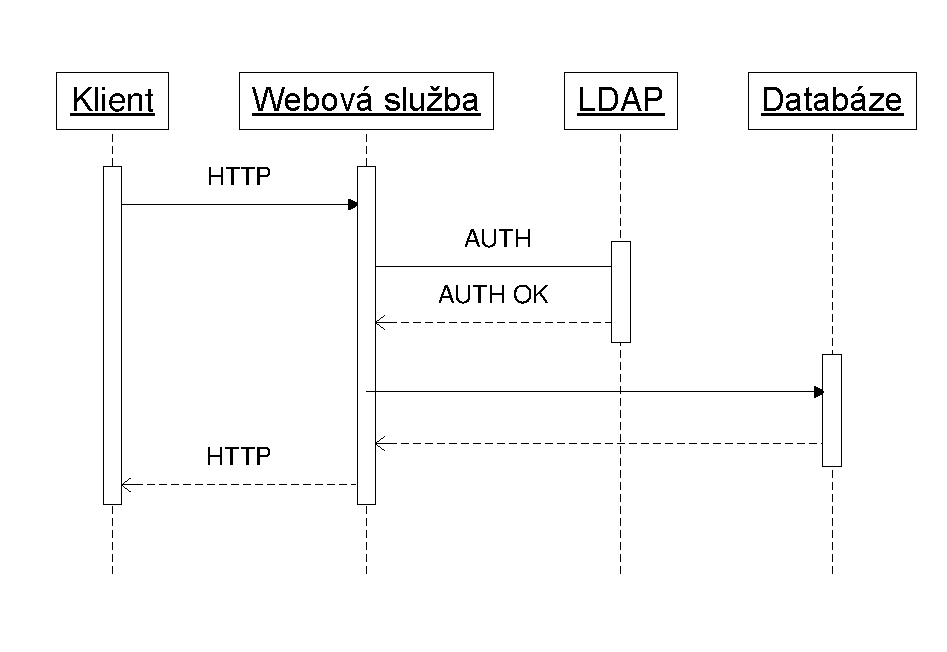
\includegraphics[scale=0.8]{visio/auth_ldap.pdf}
\caption{Diagram aktivit při úspěšné autentizaci}
\label{fig:authldap}
\end{figure}
\vspace{-6mm}
\subsection{LDAP}
 Directory Access Protocol (LDAP) je internetový protokol definující přístup k distribuované adresářové službě. Podle tohoto protokolu jsou jednotlivé položky na serveru ukládány formou záznamů a uspořádány do stromové struktury. Protokol LDAP je byl navržen v souladu  se sadou standartů X.500 vyvinutých pro adresářové služby v počítačových sítích. Protokol LDAP je jejich odlehčenou verzí.\\ \indent
Aplikace funguje na bázi klient-server. Klient se při komunikaci se serverem autentizuje. Prostřednictvím klienta lze přidávat, modifikovat a mazat záznamy na serveru.

\subsection*{Schéma}
Úkolem informačního modelu LDAP je definovat datové typy a informace, které lze v adresářovém serveru ukládat. Data jsou uchovávána ve stromové struktuře pomocí záznamů. Záznam představuje souhrn atributů (dvojice jméno - hodnota). Atributy nesou informaci o stavu daného záznamu. Záznamy, uložené v adresáři, musí odpovídat přípustnému schématu. Schéma  představuje soubor povolených objektových tříd a k nim náležících atributů.\\
Ukázka schématu definující strukturu záznamu zaměstnance:
\begin{verbatim}
objectclass ( 1.1.2.2.2 NAME 'zamestnanec'
                DESC 'zamestnanec firmy'
                SUP osoba
                MUST ( jmeno $ identifikacniCislo )
                MAY zkratkaZamestnance )
\end{verbatim}

Objekt popisující zaměstnance dědí od objektu osoba, vyžaduje povinný atribut 'jmeno' a 'identifikacniCislo' a nepovinný atribut 'zkratkaZamestnance'.

\subsection*{Funkční model}
Funkční model umožňuje pomocí základních operací manipulovat a přistupovat k záznamům v adresáři a měnit či zjišťovat tak jejich stav.
\begin{itemize}[noitemsep,nolistsep]
\item Autentizační operace: Slouží k přihlášení a odhlášení uživatele pro komunikaci s adresářovým serverem. Jsou jimi míněny především operace bind a unbind. Na úspěšném provedení operace bind závisí výsledky aktualizačních a dotazovacích operací nad adresářem.
\item Aktualizační a dotazovací operace: Každý adresářový server podporuje základní operace s daty, jako je vyhledávání, přidávání, mazání, porovnávání a modifikace záznamů. Tyto operace bývají často spjaté s nastavením bezpečnostního modelu.
\end{itemize}

\subsection*{LDAP URL}
Umístění zdroje je v LDAP specifikováno pomocí URL, které má následující tvar:
\begin{verbatim}
ldap://host:port/DN?attributes?scope?filter?extensions
\end{verbatim}
\begin{itemize}[noitemsep,nolistsep]
\item host - doména nebo IP adresa
\item port - síťový port (defaultně 389)
\item DN - význačné jméno použité jako základ pro vyhedávání
\item attributes -  seznam atributů
\item scope - specifikuje vyhledávácí rozsah  
\item filter - filtrovací kritérium
\item extensions - rozšíření
\end{itemize}

\section{Shrnutí}
Hlavním prvkem zabezpečení je VPN přístup. Uživatel bez přístupu do firemní VPN nemůže komunikovat s webovou službou. Od uživatele se očekává, že si nakonfiguruje VPN připojení v nastavení Android mobilního zařízení.\\ \indent
Použil jsem první řešení protože je shoduje se způsobem ověřování v současném systému. Stávají řešení pomocí Oracle Forms aplikace používá rovněž ověření uživatele dotazem k databázi tzn. ověření se děje na aplikační vrstvě. \\ \indent
Je nutné dívat se na pravidlo dobrovolného hesla jako na firemní pravidlo, které může být kdykoli zrušeno. V případě zrušení tohoto pravidla by se z největší pravděpodobností uplatnilo ověřování proti LDAP adresáři. 

\chapter{Webová služba}
JAX-RS citace
\section{REST}
Při návrhu REST služby jsem nejprve identifikoval všechny zdroje, které webová služba zpřístupňuje. Jedná se o údaje o docházce zaměstnanců, výkazech práce a zaměstnancích samotných. Posledním zdrojem je možnost testovat komunikaci s webovou službou. \par
Zdroj pro docházku zaměstnaců tzn. jejich příchody a odchody (označované jako události) a poskytované služby zobrazuje tabulka \ref{tab:urievents}. Služba umožňuje operace CRUD na datovém zdroji zaměstnanců a dále zjištění součtu doby v zaměstnání.

\definecolor{Gray}{gray}{0.9}
\renewcommand{\arraystretch}{1.5}
\begin{table}[H]
\begin{center}
\begin{tabular}{| m{2cm} |  m{10cm} |}
\hline
\rowcolor{Gray}
GET & events/\{icp\}?from=\{from\}\&to=\{to\} \\ \hline
&  \parbox{10cm}{Získá všechny události zaměstnance za dané období\\
Parametry:\begin{itemize}[noitemsep,nolistsep]
\item icp - identifikátor zaměstnance
\item from - datum začátku období
\item to - datum konce období
\end{itemize}} \\ \hline
\rowcolor{Gray}
DELETE  & events/\{rowid\} \\  \hline
&  \parbox{10cm}{Smaže danou událost\\
Parametry:\begin{itemize}[noitemsep,nolistsep]
\item rowid - identifikátor události
\end{itemize}} \\ \hline
\rowcolor{Gray}
POST  & events \\  \hline
&  \parbox{10cm}{Vytvoří událost, používá se bez parametrů protože identifikátor pro událost vytváří server
} \\ \hline
\rowcolor{Gray}
PUT  & events/\{rowid\} \\ 
&  \parbox{10cm}{Aktualizuje danou událost\\
Parametry:\begin{itemize}[noitemsep,nolistsep]
\item rowid - identifikátor události
\end{itemize}} \\ \hline
\rowcolor{Gray}
GET & events/sum/\{icp\}?from=\{from\}\&to=\{to\} \\ \hline
&  \parbox{10cm}{Získá součet přítomnosti zaměstnance za dané období\\
Parametry:\begin{itemize}[noitemsep,nolistsep]
\item icp - identifikátor zaměstnance
\item from - datum začátku období
\item to - datum konce období
\end{itemize}} \\ \hline
\end{tabular}
\end{center}
\caption{Služby pro události docházky}
\label{tab:urievents}
\end {table}

\noindent
Zdroj pro údaje o zaměstnancích
\begin{table}[H]
\begin{center}
\begin{tabular}{| m{2cm} |  m{10cm} |}
\hline
\rowcolor{Gray}
GET  & employees/\{icp\} \\ \hline
&  \parbox{10cm}{Získá údaje o zaměstnaci identifikovém pomocí parametru\\
Parametry:\begin{itemize}[noitemsep,nolistsep]
\item icp - identifikátor zaměstnance
\end{itemize}} \\ \hline
\hline
\rowcolor{Gray}
GET  & employees/all/\{icp\} \\ \hline
&  \parbox{10cm}{Získá seznam všech zaměstnanců, kteří jsou aktuálně v zaměstnaneckém poměru, obsahuje informaci zda jsou tito zaměstnanci podřízení, vzhledem k zaměstnanci identifikovém pomocí parametru\\
Parametry:\begin{itemize}[noitemsep,nolistsep]
\item icp - identifikátor zaměstnance
\end{itemize}} \\ \hline
\rowcolor{Gray}
GET  & employees/lastevents \\ 
&  \parbox{10cm}{Získá poslední událost v docházce všech zaměstnanců, kteří jsou aktuálně v zaměstnaneckém poměru}\\
\hline
\rowcolor{Gray}
GET  & employees/lastevents/\{icp\} \\ 
&  \parbox{10cm}{Získá poslední událost v docházce zaměstnance identifikovém pomocí parametru}\\
\hline
\end{tabular}
\end{center}
\caption{Služby pro zaměstnance}
\label{tab:uriemps}
\end{table}
\noindent

Zdroj výkazy práce
\begin{table}[H]
\begin{center}
\begin{tabular}{| m{2cm} |  m{10cm} |}
\hline
\rowcolor{Gray}
GET  &records/\{kodpra\}?from=\{from\}\&to=\{to\} \\ 
&  \parbox{10cm}{Získá všechny výkazy práce zaměstnance za dané období\\
Parametry:\begin{itemize}[noitemsep,nolistsep]
\item kodpra - identifikátor zaměstnance (zkratka)
\item from - datum začátku období
\item to - datum konce období
\end{itemize}} \\ \hline
\rowcolor{Gray}
GET & records/sum/\{icp\}?from=\{from\}\&to=\{to\} \\ \hline
&  \parbox{10cm}{Získá součet vykázaného času zaměstnance za dané období\\
Parametry:\begin{itemize}[noitemsep,nolistsep]
\item icp - identifikátor zaměstnance
\item from - datum začátku období
\item to - datum konce období
\end{itemize}} \\ \hline
\end{tabular}
\end{center}
\caption{Služby pro výkazy práce}
\label{tab:urirecords}
\end{table}

\section{Filtry}

\section{web.xml}

\section{REST}
RestaTemplates - springframework= jak to vola klient...
\begin{enumerate}
\item REST operace - davkove vs jednotlive
\item REST, tabulka URI, 
\end{enumerate}

\section{Klienti jiných platforem?}

\chapter{Android aplikace}

\section{Funkcionalita}
[TODO co uz bylo ve starem, co v novem]
Na základě současného systému a potřeb zaměstnanců byla vybrána k implementaci následující funkčnost: 

\paragraph{Docházka}
\begin{itemize}[noitemsep,nolistsep]
\item Zobrazení událostí docházky daného zaměstnance pomocí denní časové osy
\item Zobrazení událostí docházky daného zaměstnance pomocí seznamu
\item Uživatel má možnost přidávat, editovat a mazat svoje události
\item Aplikace zajišťuje automatickou synchronizaci těchto údajů s firemní databází
\item Zobrazení poměru typů docházkových událostí za dané období pro vybraného zaměstnance
\item Zobrazení vývoje daného typu události v daném období pro vybraného zaměstnance
\item Zobrazení souhrných statistik událostí za dané období pro vybraného zaměstnance
\end{itemize}

\paragraph{Výkazy práce}
\begin{itemize}[noitemsep,nolistsep]
\item Zobrazení seznamu výkazů za dané období pro vybraného zaměstnance
\item Zobrazení poměru typů zakázek za dané období pro vybraného zaměstnance
\item Zobrazení vývoje daného typu zakázky v daném období pro vybraného zaměstnance
\item Zobrazení souhrných statistik výkazů za dané období pro vybraného zaměstnance
\end{itemize}

\newpage
\paragraph{Aktuální přítomnost na pracovišti}
\begin{itemize}[noitemsep,nolistsep]
\item Zobrazení seznamu všech zaměstnanců a jejich poslední docházkové události  (aktuální stav přítomnosti či nepřítomnosti na pracovišti)
\item Uživatel má možnost spravovat seznam svých oblíbených zaměstnanců a tento seznam zobrazovat přednostně
\end{itemize}

\paragraph{Widgety}
\begin{itemize}[noitemsep,nolistsep]
\item Widget pro rychlé zadání docházkové události
\item Widget pro zobrazení poslední docházkové události vybraného zaměstnance (aktuální stav přítomnosti či nepřítomnosti na pracovišti)
\end{itemize}

\paragraph{Notifikace}
\begin{itemize}[noitemsep,nolistsep]
\item Notifikace při opomenutí zadání příchodu či odchodu
\end{itemize}

\paragraph{Online vs offline}\mbox{}\\ \\ \indent
Veškeré výše zmíněné funkce jsou dostupné jak v režimu online tak i offline. Rozdíl je v tom, že v režimu offline nemusí aplikace pracovat s aktuálními daty.

\subsection{Nastavení a konfigurovatelnost}
Zařízení si musí pamatovat údaje nutné pro snadnou obsluhu tzn. uživatelské jméno a heslo. V následujícím seznamu je výčet všech konfigurovatelných vlastností aplikace:

\begin{itemize}[noitemsep,nolistsep]
\item Parametry připojení k webové službě (doména a port)
\item Povolení automatické synchronizace pouze při WIFI připojení
\item Perioda synchronizace vlastních docházkových událostí
\item Perioda synchronizace widget pro zobrazení vybraných zaměstnanců
\item Perioda synchronizace seznamu zaměstnanců
\item Upozornění na chybějící příchod (vypnout či zapnout)
\item Upozornění na chybějící odchod (vypnout či zapnout)
\item Časová prodleva pro upozornění na chybějící událost docházky
\item Barva typu docházkové události
\item Barva typu zakázky
\end{itemize}

\subsection{Uživatelská přívětivost}
Uživatelské rozhraní aplikace klade důraz na přehlednost, ergonomii a časově efektivní obsluhu.[TODO jeste neco vymyslet]
\subsection{Návrhy na vylepšení}
Původní ambicí byla možnost zadavání výkazů práce. Vzhledem k tomu, že taková funkčnost by vyžadovala změny v současném systému, bylo od tohoto záměru upuštěno. Kromě zadávání výkazů práce by bylo možné rovněž vykazovat do knihy jízd.\\ \indent
Velikým přínosem by byla možnost vytváření šablon pro často opakované výkazy, která by uživateli ušetřila nezanedbatelné množství času.\\ \indent
Posledním vylepšením by byla možnost rychlého zavolání přímo z profilu vybraného zaměstnance.

\section{Výběr podporovaných verzí Android zařízení}

\section{Komponenty Android aplikace}

\subsection{Activity}
Aktivita představuje jednu obrazovku s uživatelským rozhraním. Každá akvitita umožňuje nějakou funkčnost. Příkladem aktivit použitých v implementované aplikaci může být zobrazení denní docházky uživatele, kalendář umožňující výběr data, přidání a editace docházkové události nebo uživatelské nastavení.

\subsubsection*{Životní cyklus aktivity}
Aktivita se může nacházet ve třech stavech:

\begin{itemize}[]
\item \textbf{Běžící}\\
Aktivita je na popředí a umožňuje interakci s uživatelem.
\item \textbf{Pozastavený}\\
Na popředí se dostala jiná aktivita. Pozastavená aktivita je stále viditelná, ale je překrytá novou aktivitou. Pozastavená aktivita nemůže provádět interakci s uživatelem. Objekt aktivity zůstává v paměti, je zachována veškerá stavová informace. Při nedostatku systémové paměti může být aktivita zničena.
\item \textbf{Zastavený}\\
Aktivita není viditelná. Objekt aktivity zůstává v paměti, je zachována veškerá stavová informace. Při nedostatku systémové paměti může být aktivita zničena.
\end{itemize}

\subsubsection*{Metody životního cyklu aktivity}
Při přechodech aktivity mezi výše uvedenými stavy dochází k volání callback metod. Tyto metody jsou volány systémem. Každá  
z metod má defaultní chování. Programátor může libovolnou z metod překrýt v případě, že požaduje jinou funkcionalitu, ale musí mít na paměti, že většina z nich vyžaduje volání metody rodiče.
\begin{itemize}[]
\item \textbf{onCreate()}\\
Metoda je volána v okamžiku, kdy je aktivita poprvé vytvořena. Zde se připraví prvky uživatelského rozhraní a nastaví se zdroje dat. Pokud existuje uložený stav aktivity z dřívější doby, může být využit. 
\item \textbf{onRestart()}\\
Volána pokud se aktivita před tím nacházela ve stavu \emph{Zastavený} a má se dostat do stavu \emph{Běžící}.
\item \textbf{onStart()}\\
Volána před tím, než se aktivita stane viditelnou.
\item \textbf{onResume()}\\
Volána před tím, než je uživatelovi umožněna interakce s aktivitou. Aktivita se dostává na vrchol zásobníku aktivit aplikace.
\item \textbf{onPause()}\\
Volána ve chvíli kdy se má jiná aktivita dostat na popředí. V této metodě by měla být uložena veškerá rozpracovaná data a ukončeny úkoly, které si zabírají výpočetní výkon. Nová aktivita není spuštěna, dokud tato metoda není dokončena.
\item \textbf{onStop()}\\
Po volání metody není aktivita nadále viditelná. K volání dochází v situaci, kdy je aktivita ukončována nebo se jiná aktivita dostala do popředí.
\item \textbf{onDestroy()}\\
Volání před tím než je aktivita ukončena. K volání dochází v případě, že aktivita končí svoji činnost nebo v situaci, kdy se systém dožaduje systémových prostředků.
\end{itemize}

\subsubsection*{Ukládání stavu aktivity}
Ukládat stav aktivity je vhodné protože systém může zničit aktivitu z důvodu nedostatku paměti. Další důvodem je situace, kdy uživatel změní orientaci obrazovky. V takové situaci nezůstává v paměti objekt aktivity, ale aktivita musí být znovu vytvořena. Uživatel samozřejmě očekává, že aktivitu nalezne ve stejném stavu v jakém ji opustil. K těmto účelům jsou určeny dvě callback metody:

\begin{itemize}[]
\item \textbf{onSaveInstanceState(Bundle)}\\
Metoda je volána před tím než je aktivita zničena (před provedením \emph{onStop()}. Do objektu \emph{Bundle} by měla být uložena všechna data, která jsou nutná pro obnovu předchozího stavu aktivity. Data jsou ukládána ve formátu klíč-hodnota. Metoda není volána v situaci, kdy uživatel explicitně ukončil aktivitu. Na začátku metody je nutné zavolat metodu rodiče, aby mohl být uložen stav prvků UI pomocí defaultní implementace.
\item \textbf{onRestoreInstanceState(Bundle)}\\
Metoda je volána (po provedením \emph{onStart()}) v případě, že aktivita byla znovuobnovena z předchozího uloženého stavu.Na začátku metody je nutné zavolat metodu rodiče, aby mohl být obnoven stav prvků UI pomocí defaultní implementace.
\end{itemize}
[TODO UML class diagram]

\subsection{Fragment}
Fragment představuje komponentu uživatelského rozhraní, která je součástí aktivity. Aktivita může obsahovat více fragmentů a fragment může být využíván ve více aktivitách. Jedná se tedy o modul umožňující nějakou funkčnost, který má vlastní životní cyklus, přijímá události z uživatelského rozhraní a může být přidán či odstraněn z aktivity během její činnosti. Fragment musí být vždy součástí nějaké aktivity a je přímo ovlivňován životním cyklem hostující aktivity.\\ \indent
K vytvoření fragmentu je nutné oddědit od třídy \emph{android.app.Fragment}. 

\subsubsection*{Metody životního cyklu fragmentu}
Tato třída je podobná třídě aktivity s tím rozdílem, že obsahuje několik metod životního cyklu navíc:
\begin{itemize}[]
\item \textbf{onAttach()}\\
Metoda je volána jakmile je fragment přiřazen k aktivitě. 
\item \textbf{onCreateView()}\\
Volána poté co je fragment vytvořen. Fragment který má uživatelské rozhraní musí vrátit objekt \emph{View}, který obsahuje uživatelské rozhraní pro tento fragment.
\item \textbf{onActivityCreated()}\\
Volána ve chvíli, kdy je vytvořena hostující aktivita.
\item \textbf{onDestroyView()}\\
Volána ve cvhíli, kdy je uživatelské rozhraní fragment odstraňováno.
\item \textbf{onDetach()}\\
Volána ve chvíli, kdy je fragment odstraňován z aktivity.
\end{itemize}
[TODO priklady fragmentu z projektu]
\subsubsection*{Provádění transakcí}
Fragment je možné přidávat, mazat či nahrazovat jinou v rámci rodičovské aktivity. Ty akce se nazývají transakce a provádějí se pomocí třídy \emph{FragmentTransaction}.V následující ukázce kódu je současný fragment v aktivitě nahrazen fragmentem \emph{PieChartFragment} zobrazující koláčový graf. Ukázka je ze třídy \emph{ChartActivity}:

\begin{lstlisting}
FragmentTransaction ft = getSupportFragmentManager().beginTransaction();
PieChartFragment pieFragment = new PieChartFragment();
ft.replace(R.id.displayChart, pieFragment, FRAG_PIE);
ft.setTransition(FragmentTransaction.TRANSIT_FRAGMENT_CLOSE);
ft.commit();
\end{lstlisting}

\subsubsection*{Změna konfigurace s využitím fragmentu}
Další uplatnění fragmentů se nachází v ošetření situace, kdy se v důsledku rotace zařízení změní poloha displeje. V případě kdy aktivita spouští asynchronní úkol (\emph{Asynctask} \ref{sec:asynctask}) a uživatel otočí displej, aktivita bude restartována. V momentě kdy \emph{Asynctask} dokončí svůj úkol bude jeho výsledek zasílat staré instanci aktivity, která v té chvíli už neexistuje. Kromě toho nově vytvořená aktivita spustí znovu ten samý \emph{Asynctask}. Obojí je samozřejmě nežádoucí. Řešením tohoto problému je využít fragment jako hostitele pro \emph{Asynctask} a nastavit metodou fragmentu \emph{setRetainInstance (true)} vlastnost, že fragment nebude restartován při restartu jeho hostitelské aktivity\cite{config}. 
[TODO odkazat se na tridy v projektu nebo dat ukazku do prilohy]

\subsection{Async task}
\label{sec:asynctask}
\emph{AsyncTask} je komponenta sloužící k provedení operace paralelně k UI (User Interface) vláknu. Třída umožňuje provedení operace na pozadí a publikování jejích výsledků na UI vlákně bez manipulace s vlákny. 
\subsubsection*{Generické parametry pro \emph{AsyncTask}}
\begin{enumerate}[noitemsep,nolistsep]
\item \textbf{Params} typ parametrů předaných úkolu před provedením.
\item \textbf{Progress} typ jednotek pro průběh operace publikovaných během výpočtu na pozdaí.
\item \textbf{Result} typ pro výsledek výpočtu. 
\end{enumerate}

\subsubsection*{Metody \emph{AsyncTask}}
Třída \emph{AsyncTask} využívá těchto metod:
\begin{itemize}[]
\item \textbf{onPreExecute()}\\
volána na UI (User Interface) vlákně před tím, než je úkol spuštěn. Metoda louží k přípravě asynchronní akce např. zobrazení dialogu s průběhem akce.
\item \textbf{doInBackground(Params...)}\\
provádí se ve vlastním vlákně na pozadí. Vrací výsledek svojí akce. Může oznamovat průběh akce pomocí \emph{ publishProgress(Progress...)}.
\item \textbf{onProgressUpdate(Progress...)}\\
volána na UI vlákně. Slouží k zobrazení průběhu akce zatímco úkol na pozadí je stále prováděn.
\item \textbf{onPostExecute(Result)}\\
volána na UI vlákně po tom, co je úkol na pozadí dokončen. Výsledek akce na pozadí je předán jako parametr.
\end{itemize}

\emph{AsyncTask} komponenty jsou vhodné pro krátké operace (max jednotky sekund), které přímo ovliňují chování uživatelského rozhraní. Příkladem takové operace může být stažení dat, která mají být zobrazena okamžitě jakmile jsou dostupná. Taková akce musí být provedena asynchronně jinak by docházelo k efektu zamrzání uživatelského rozhraní.
[TODO priklady AsyncTask z projektu+diagram trid]

\subsection{Service}
\emph{Service} neboli služba je komponenta aplikace, která provádí dlouhotrvající operaci na pozadí a neposkytuje uživatelské rozhraní. Služba může být spuštěna vlastní aplikací, z jiné aplikace či systémovou komponentou.  Služba běží v hlavním vlákně hostujícího procesu. Služby lze klasifikovat na dva typy:

\begin{description}[]
\item \textbf{Started}\\
Spuštěná služba, je taková služba, která byla spuštěna voláním metody \emph{startService()} kontextu komponenty. Služba běží na pozadí dokud neskončí svojí činnost, a to i tehdy pokud byla spouštějící komponenta zničena. Služba typicka provádí nějakou operaci, bez interakce se spouštějící komponentou a po dokončení se sama zničí. Metody životního cyklu služby jsou: 
\begin{itemize}[]
\item \textbf{onCreate()}\\
Volána ve chvíli kdy je služba vytvořena. Je určena k počáteční inicializaci.
\item \textbf{onStartCommand()}\\
Volána ve chvíli kdy je služba spuštěna. Metodou \emph{stopSelf()} se může služba sama ukončit.
\item \textbf{onDestroy()}\\
Volána systémem ve chvíli, kdy je služba ničena. Určena pro uvolnění zdrojů.
\end{itemize}
\item \textbf{Bound}\\
Připoutaná (angl. bound) služba, je taková služba, ke které se komponenta připoutala voláním \emph{bindService()}. Připoutaná služba poskytuje klient-server rozhraní, které umožnuje komunikaci s touto službou pomocí meziprocesové komunikace. Služba běží pouze pokud je k ní nějaká komponenta svázaná. Ke službě může být připoutáno více komponent, jakmile se všechny odpoutají, je služba zničena. Metody životního cyklu služby jsou kromě \emph{onCreate()}, \emph{onDestroy()} tyto:
\begin{itemize}[]
\item \textbf{onBind()}\\
Volána systémem ve chvíli, kdy se jiná komponenta chce ke službě přivázat voláním \emph{bindService()}. Vrací objekt \emph{IBinder}, který představuje rozhraní pro komunikaci.
\item \textbf{onUnbind()}\\
Komponenta klienta se odpoutává od služby.
\end{itemize}
\end{description}
[TODO priklady v projektu]
\subsection{Content provider}
\emph{Content provider} je jedna ze základních komponent pro tvorbu Android aplikace. Komponenta řídí přístup k centrálnímu úložišti dat představující SQLite databázi. \emph{Content provider} zapouzdřuje data a poskytuje je ostatním aplikacím pomocí \emph{android.content.ContentResolver} rozhraní. Pokud data aplikace nemají být přístupná i jiným aplikacím, není této komponenty potřeba a je možné přistupovat k datům přímo pomocí třídy \emph{android.database.sqlite.SQLiteDatabase}. Důležité metody této komponenty jsou::

\begin{itemize}[]
\item \textbf{query()}\\
Provádí dotaz do úložiště a vrací výsledek dotazu.
\item \textbf{insert()}\\
Vlkádá data do úložiště.
\item \textbf{update()}\\
Aktualizuje existující data v úložišti.
\item \textbf{delete()}\\
Maže data z úložiště.
\item \textbf{getType()}\\
Vrací MIME typ dat obsažených v úložišti.
\end{itemize}

\subsection*{Přístup pomocí URI}
Umístění dat je specifikováno pomocí URI. Ukázka URI použitého v aplikaci:
\begin{verbatim}
content://user_dictionary/words
\end{verbatim}
\begin{itemize}[noitemsep,nolistsep]
\item \textbf{content://} představuje schéma
\item \textbf{dictionary} symbolické jméno úložiště tzv. \emph{authority}
\item \textbf{words} název tabulky
\end{itemize}

\subsection{Broadcast receiver}
Komponenta \emph{Broadcast receiver} slouží jako posluchač systémové či aplikační události. Všichni registrovaní posluchači jsou informováni jakmile událost nastane. Objekt musí být registrován pomocí \emph{android.content.Context.registerReceiver()} metody kontextu k poslechu události specifikované pomocí filtru událostí \emph{android.content.IntentFilter}. Událost může být vyvolána systémem (např. připojení nabíječky, změna stavu připojení k síti) nebo může být vytvořena aplikací. Nejdůležitější metoda této třídy:
\begin{itemize}[]
\item \textbf{onReceive(Context context, Intent intent)}\\
Metoda je volána ve chvíli kdy je přijata očekávaná událost. Životnost objektu po dokončení této metody končí.
\end{itemize}
[TODO priklad z applikace]
\subsection{Loader}
Třída \emph{android.content.Loader<D>} slouží k asynchronnímu načtení dat pro aktivitu či fragment. Monitoruje zdroj svých dat a automaticky se aktualizuje v momentě změny těchto dat. Loader spolupracuje s třídami \emph{	android.app.LoaderManager}, která řídí činnost všech Loader objektů patřících dané aktivitě či fragmentu. Aktivita či fragment musí implementovat rozhraní \emph{android.app.LoaderManager.LoaderCallbacks<D>}, které obsahuje tyto callback metody:

\begin{itemize}[]
\item \textbf{onCreateLoader (int id, Bundle args)}\\
Určená pro inicializaci Loader objektu s daným \emph{id}.
\item \textbf{onLoadFinished (Loader<D> loader, D data)}\\
Volána po načtení dat. Poskytuje objekt s načtenými daty.
\item \textbf{onLoaderReset (Loader<D> loader)}\\
Volána v případě kdy Loader byl resetován. Určena pro zrušení všech referencí na zdrojový objekt s daty.
\end{itemize}


\subsection{Alarm manager}
Třída \emph{android.app.AlarmManager} je určená pro případy kdy má nějaká akce proběhnout v určený čas a to i v případě kdy aplikace není spuštěna. Ve chvíli kdy je akce prováděna \emph{AlarmManager} drží zámek CPU do té doby než akce skončí. Volitelně lze nastavit, zda se má kvůli provedení akce vzbudit zařízení z režimu spánku.
\begin{itemize}[]
\item \textbf{setRepeating(int type, long triggerAtMillis, long intervalMillis, PendingIntent operation)}\\
Naplánuje pravidelně se opakující akci.
\item \textbf{set(int type, long triggerAtMillis, PendingIntent operation)}\\
Naplánuje akci na učitý čas.
\end{itemize}

[TODO ukázka kódu + popis pouziti]

\section{Komponenty pro synchronizaci}
Pro synchronizaci je klíčovou komponentou třída \emph{android.content.\\AbstractThreadedSyncAdapter}. Třída provádí akci na pozadí ve vlastním vlákně. Synchronizace je vyvolána systémovou komponentou \emph{android.content.SyncManager}, v závislosti konkrétním nastavení pro konkrétní adaptér. Odpadá tak starost s práci s vlákny a k využití této komponenty stačí implementovat metodu \emph{onPerformSync()}:
\begin{itemize}[]
\item \textbf{onPerformSync(Account account, Bundle extras, String authority, ContentProviderClient provider, SyncResult syncResult)}\\
\begin{itemize}[]
\item  \textbf{account} účet, který je synchronizován
\item  \textbf{extras} parametry specifické pro tento adaptér
\item  \textbf{authority} \emph{authority}, pro kterou je požadována synchronizace
\item  \textbf{provider} instance \emph{ContentProviderClient}, která odkazuje na \emph{ContentProvider} pro tuto \emph{authority}
\item  \textbf{syncResult} určeno pro výsledek synchronizace, který bude předán komponentě \emph{SyncManager}
\end{itemize}
\end{itemize}
[TODO priklad z applikace]
[TODO diagram komponent]
\section{Uživatelský účet}
Android poskytuje správu účtů pro online služby. Uživatel zadá svoje přihlašovací údaje při vytvoření účtu a dává tak aplikaci svolení k využívání tohoto účtu.\\ \indent
Různé online služby mohou využívat odlišný způsob pro autentizaci. Android manažer účtů využívá kompomentu \emph{authenticator} \cite{accman}, která je obvykle poskytována třetí stranou - poskytovatelem dané služby. Příkladem služby, která poskytuje vlastní \emph{authenticator} je např. Google, Facebook a Microsoft Exchange.\\ \indent
Nejdůležitější třída pro práci s účty je \emph{AccountManager}. Zde je výčet nejdůležitějších metod:
\begin{itemize}[]
\item \textbf{addAccountExplicitly(Account account, String password, Bundle userdata)}\\
Vytvoří nový účet.
\item \textbf{Account[]: getAccountsByType(String type)}\\
Vrátí seznam všech účtů daného typu.
\item \textbf{setAuthToken(Account account, String authTokenType, String authToken)}\\
Přidá autentizační token do cache paměti pro daný účet.
\item \textbf{String:getPassword(Account account)/setPassword(Account account, String password)}\\
Získání uloženého hesla pro účet./Nastavení hesla.
\end{itemize}

Na diagramu \ref{obr:andauth} je zobrazen průběh vytvoření účtu, který je použit v implementované aplikaci. Jakmile uživatel v sekci \emph{Nastavení->Účty} (obr. \ref{obr:setting}) zvolí přidání nového účtu a následně zvolí typ účtu (obr. \ref{obr:addacc}), manažer účtů spustí službu \emph{AutheticationService}. Služba vytvoří instanci třídy \emph{AccountAuthenticator} - \emph{authenticator} komponenty. \emph{AccountManager} následně volá metodu \emph{addAccount()}, která zkontroluje zda již účet daného typu existuje. Pokud ne, vrací objekt \emph{Bundle} obsahující \emph{Intent} s klíčem \emph{AccountManager.KEY\_INTENT} označující, že bude nutná interakce s uživatelem. Následně je spuštěna aktivita \emph{AuthenticatorActivity} vyzývající uživatele, aby zadal svoje přihlašovací údaje. Po potvrzení je vytvořen účet (obr. \ref{obr:setting}).
\begin{figure}[H]
  \centering
  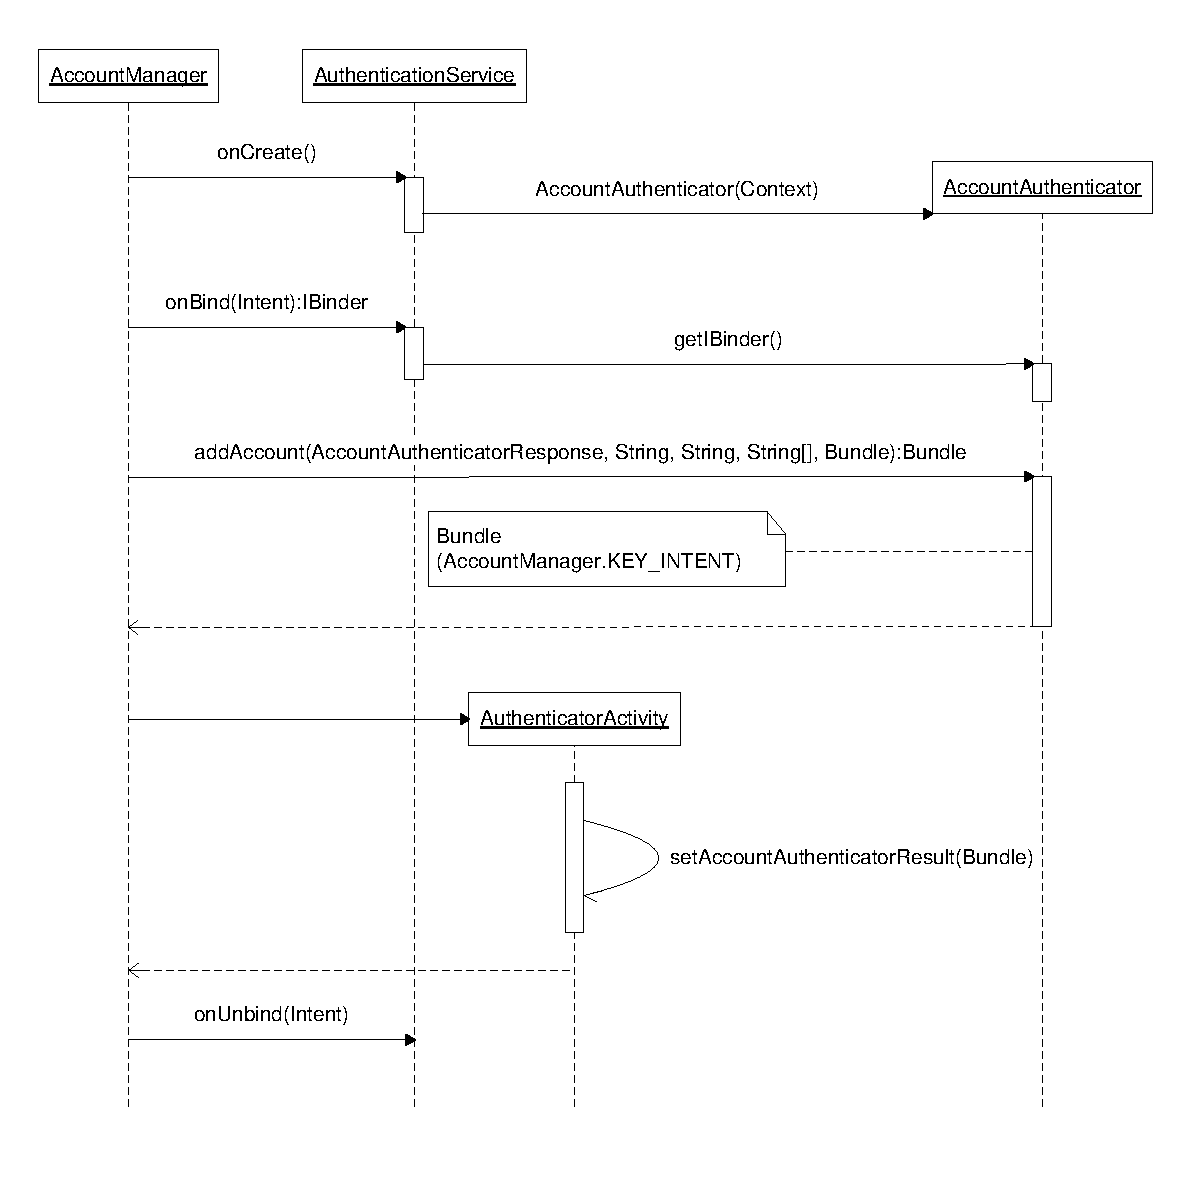
\includegraphics[scale=0.7]{visio/andauth.pdf}
\caption{Sekvenční diagram zobrazující průběh vytvoření účtu}
\label{obr:andauth}
\end{figure}

\begin{figure}[H]
\centering
\begin{minipage}{.5\textwidth}
  \centering
  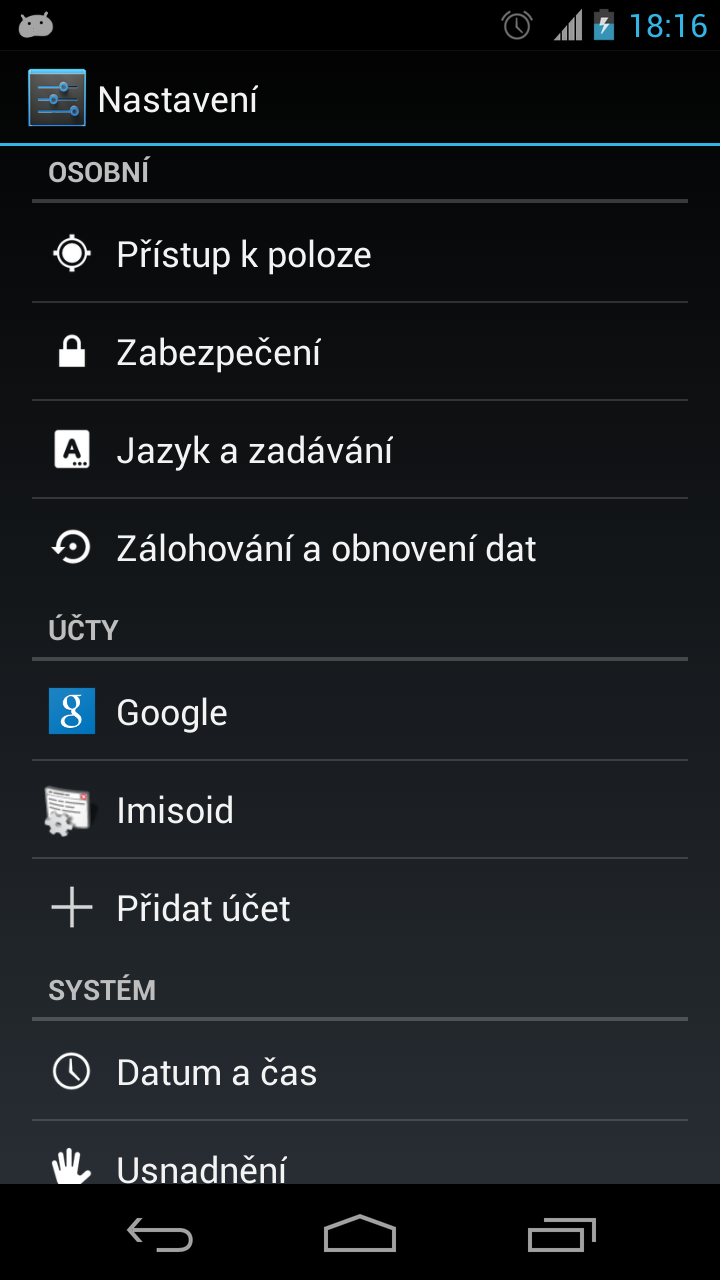
\includegraphics[width=.75\linewidth]{scr/setting.png}
  \captionof{figure}{Nastavení}
  \label{obr:setting}
\end{minipage}%
\begin{minipage}{.5\textwidth}
  \centering
  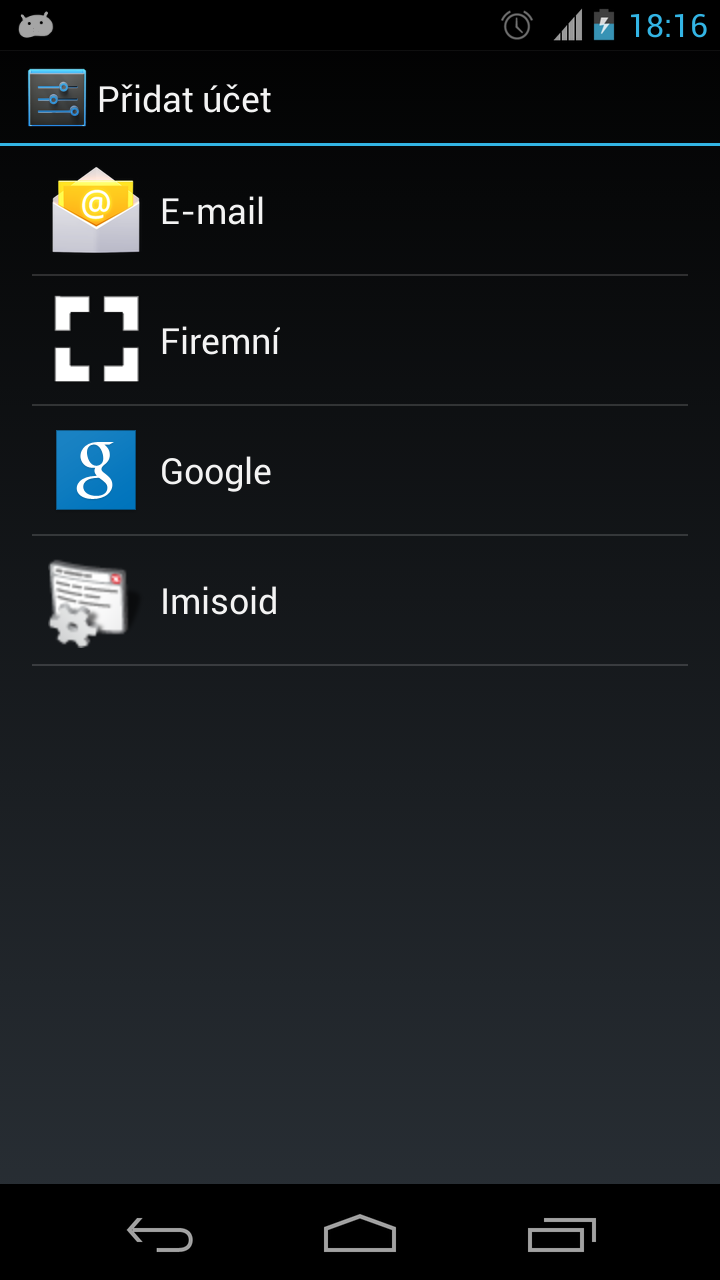
\includegraphics[width=.75\linewidth]{scr/addacc.png}
  \captionof{figure}{Přidání účtu}
  \label{obr:addacc}
\end{minipage}
\end{figure}



[TODO obr s aktivitou]
\section{Ukládání dat}
Android umožňuje několik způsobů jak persistentně ukládat data aplikace. Programátor by měl vzít v úvahu, zda data mají být soukromá či dostupná i ostatním aplikacím a také velikost těchto dat. 
\subsection*{Sdílené preference} Ukládá primitivní datové typy ve tvaru klíč-hodnota. Slouží k uložení nastavení specifických pro aplikaci. K těmto se přistupuje pomocí \emph{SharedPreferences} rozhraní. Data jsou ukládána persistentně. \\ V aplikaci používám toto úložiště pro nastavení síťového připojení, barevného nastavení pro typy docházkových událostí a další uživatelsky měnitelné hodnoty.\\ \\
Objekty se získávají pomocí příslušné get metody:
\begin{lstlisting}
SharedPreferences settings = PreferenceManager.getDefaultSharedPreferences(context);
int color = settings.getInt("color", defaultColor);
\end{lstlisting}

\noindent
Změny nastavení se provádějí pomocí \emph{SharedPreferences.Editor} rozhraní, které se postará aby data zůstala konsistentní a řídí transkační zpracování.\\
\begin{lstlisting}
SharedPreferences settings = PreferenceManager.getDefaultSharedPreferences(context);
SharedPreferences.Editor editor = settings.edit();
editor.putInt(("color", userColor);
editor.commit();
\end{lstlisting}

\subsection*{Interní úložiště}
Soubory lze ukládat v interní paměti zařízení. Tyto soubory jsou defaultně přístupné pouze pro aplikace, která je vytvořila a při odinstalování jsou automaticky smazány.
\subsection*{Externí úložiště}
Další možností pro ukládání souborů je externí úložiště (např. SD karta).  Toto úložiště je sdílené a data mohou být editována i mimo aplikaci.
\subsection*{SQLite databáze}
Data lze ukládat persistentně pomocí SQLite databáze. Vytvořená databáze je dostupná jakkékoli třídě v aplikaci, ale není přístupná mimo aplikaci, která jí vytořila. SQLite databázi detailněji popisuji v kapitole \ref{sqlite}.
[TODO citace]

%\subsection{SQLite}
%\label{sqlite}
[TODO]je treba resit delku dat napriklad stringu?, dynamic typing
[TODO rozepsat podrobneji]


\section{Vlastní  komponenta UI}
+ 9png grafika

\section{Widgety}

\section{GPS + mapy}

\begin{itemize}[noitemsep,nolistsep]
\item  \textbf{READ\_GSERVICES}
\end{itemize}

\begin{itemize}[noitemsep,nolistsep]
\item  \textbf{MAPS\_RECEIVE}
\end{itemize}

\section{Notifikace}

\section{Zpětná kompatibilita + support balíček?}
význam support package, nějaký příklad proč ho v mojí aplikaci potřebuji
\section{Vytváření grafů}
Pro potřebu přehledného zobrazení statistik jsem se rozhodl využít grafy. Konkrétně koláčový graf pro zobrazení poměrů typů docházkových událostí či zakázek a sloupcový graf pro zobrazení jejich vývoje v čase.

\subsection*{Implementace vlastní komponenty}
Implementace vlastních komponent pro grafy by bylo velice časově náročné a proto jsem tuto variantu zamítl.

\subsection*{Využití cloudového řešení}
Jako cloudové řešení se nabízí Google Charts API\cite{googlecharts}. Google Charts API poskytuje Javascriptové knihovny, pro vygenerování grafu. Aplikace stáhne knihovny, které potřebuje pro požadový graf, vytvoří objekt grafu, naplní ho daty, upraví jeho parametry a nakonec ho umístí do \emph{android.webkit.WebView} komponenty, která slouží k zobrazení webového obsahu. Nevýhoda použití Google Charts API spočívá v nedostupnosti jakýchkoli grafů při nedostupnosti síťového připojení. Na obr. \ref{fig:gcharts} je ukázka grafu.
\begin{figure}[H]
  \centering
  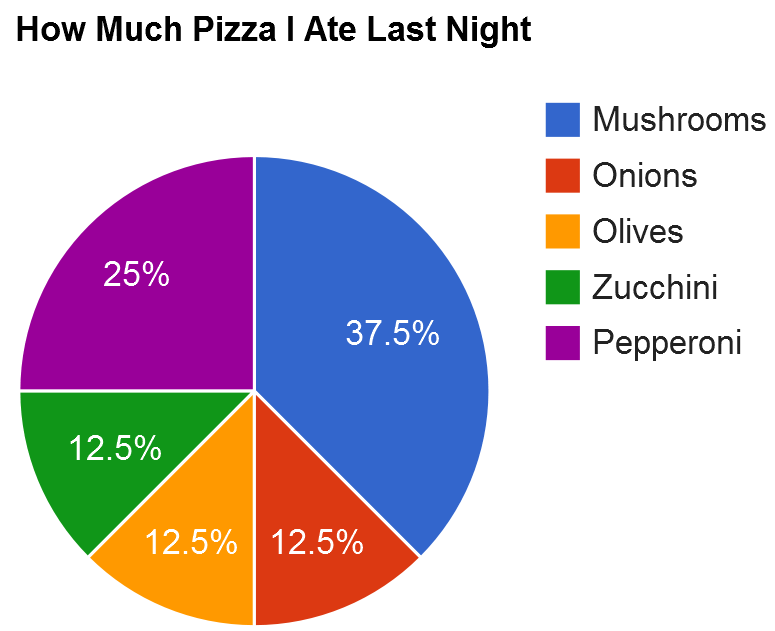
\includegraphics[scale=0.5]{obr/gcharts.png}
\caption{Ukázka grafu vytvořeného Google Charts API}
\label{fig:gcharts}
\end{figure}
\subsection*{Použití knihovny třetí strany}
Jako nejlepší řešení jsem vyhodnotil použití knihovny třetí strany konkrétně AChartEngine \cite{achartengine} ve verzi 1.1.0. Výhoda tohoto řešení spočívá v tom, že s grafy lze pracovat i pokud je zařízení mimo dosah sítě.
[TODO obr z aplikace]


\section{Oprávnění}
V operačním systému Android běží každá aplikace ve svém \emph{sandboxu}, což je bezpečnostní mechanismus, který slouží pro oddělování běžících procesů. Pokud chce aplikace přístup k k systémovým zdrojům, datům jiné aplikace či soukromým datům uživatele musí o to explicitně požádat. To se děje prostřednictvím oprávnění (angl. permissions) staticky deklarovaných v pomocí tagu \emph{<uses-permission>} v souboru manifestu (AndroidManifest.xml). Při instalaci aplikace je uživateli zobrazen seznam všech těchto oprávnění, které aplikace požaduje a bez jeho souhlasu nemůže být aplikace naistalována. Níže je seznam všech oprávnění, které aplikace vyžaduje:
[TODO jeste ty pro mapy]
\begin{itemize}%[noitemsep,nolistsep]
\item  \textbf{ACCESS\_FINE\_LOCATION}\\
Povoluje aplikaci přístup k přesné pozici ze zdrojů GPS, vysílačů operátora či Wi-Fi.
\item  \textbf{ACCESS\_NETWORK\_STATE}\\
Povoluje aplikaci přístup k informaci o sítích.
\item  \textbf{AUTHENTICATE\_ACCOUNTS}\\
Povoluje aplikaci autentizovat vlastní účty.
\item  \textbf{GET\_ACCOUNTS}\\
Povoluje aplikaci přístup k seznamu účtů v zařízení.
\item  \textbf{INTERNET}\\
Povoluje aplikaci přístup k síťovým službám.
\item  \textbf{MANAGE\_ACCOUNTS}\\
Povoluje aplikaci přístup ke správě účtu uživatele.
\item  \textbf{READ\_SYNC\_SETTINGS}\\
Povoluje aplikaci přístup k číst nastavení pro synchronizaci.
\item  \textbf{READ\_SYNC\_STATS}\\
Povoluje aplikaci přístup ke čtení statistik synchronizace.
\item  \textbf{RECEIVE\_BOOT\_COMPLETED}\\
Povoluje aplikaci získat oznámí při restartu zařízení.
\item  \textbf{USE\_CREDENTIALS}\\
Povoluje aplikaci přístup ke přihlašovacím údajům uživatele.
\item  \textbf{VIBRATE}\\
Povoluje aplikaci požadovat vibraci zařízení.
\item  \textbf{WRITE\_EXTERNAL\_STORAGE}\\
Povoluje aplikaci přístup ke sdílenému úložišti.
\item  \textbf{WRITE\_SYNC\_SETTINGS}\\
Povoluje aplikaci měnit nastavení pro synchronizaci.
\end{itemize}


\section{Distribuce aplikace}
Vzhledem k tomu, že aplikace je určena pro použití v soukromé společnosti, je základním požadavkem její neveřejná distribuce. Standartní cesta publikováním aplikace na Google play tedy není vhodná a namísto ní jsem zvolil alternativní službu Appkilt Market\cite{appkilt}. Služba Appkilt umožňuje soukromou distribuci aplikace pomocí www odkazu ke stažení aplikace. Mimo to ještě umožnuje automatickou aktualizaci aplikace po vydání nové verze a reportování chyb na účet vývojáře. \\ \\Zde je výčet parametrů bezplatné verze služby:
\begin{itemize}[noitemsep,nolistsep]
\item 500 stažení za měsíc
\item 100 chybových reportů za měsíc
\item 1 účet administrátor
\end{itemize}

\subsection*{Verze aplikace}
Informace o verzi aplikace je nutná aby bylo možné provádět aktualizace. Verze aplikace se definuje pomocí atributů v souboru manifestu:
\begin{itemize}[noitemsep,nolistsep]
\item \textbf{android:versionCode}
Celočíselná hodnota reprezentující verzi aplikačního kódu, relativní k ostatním verzím. Hodnota by měla být zvýšena při každém vydání nové aplikace a díky tomu mohla být provedena aktualizace.
\item \textbf{android:versionName}
Řetězcová reprezentace verze určená pro uživatele. 
\end{itemize}

\subsection*{Aktualizace aplikace}
K tomu aby bylo možné využívat funkci automatické aktualizace je nutné přidat následující kód do každé aktivity aplikace, kde má být prováděna kontrola dostupnosti nové verze. Předpokladem je přítomnost potřebné knihovny \emph{AppKiltLib.jar} v projektu.
\begin{lstlisting}
@Override
protected void onPause() { 
	super.onPause();

	AppKilt.onUpdateableActivityPause();
}

@Override
protected void onResume() {
	super.onResume();
	
	AppKilt.onUpdateableActivityResume(this);
}
\end{lstlisting}

\subsection*{Podepsání aplikace}
Android systém vyžaduje aby všechny instalované aplikace byly digitálně podepsány certifikátem, který patří vývojáři aplikace. Soukromý klíč si vygeneruje sám vývojář pomocí dostupných prostředků. Před vydáním aplikace je nutné podepsat distribuovaný balík tímto soukromým klíčem.

\subsection*{Reportování chyb}
K tomu aby bylo možné využívat funkci reportování chyb je nutné přidat do projektu vlastní implementaci třídy \emph{android.app.Application} a v ní volat funkci \emph{AppKilt.init(this, "ID")}, kde řetězce \emph{ID} bude nahrazen skutečným identifikátorem přiděleným aplikaci službou AppKlit. Předpokladem je přítomnost potřebné knihovny \emph{AppKiltLib.jar} v projektu. Nevýhodou je skutečnost, že chybový report je odesílán pouze pokud je zařízení připojeno k síti v momentě kdy dojde k chybě v aplikaci, jinak se tato informace ztratí. 
\begin{lstlisting}
public class MyApplication extends Application {

	@Override
	public void onCreate() {
		super.onCreate();
		
		AppKilt.init(this, "ID");
	}
}
\end{lstlisting}


\chapter{Testování? cca 2stranky}
[TODO testovaci scenare synchronizace]
[TODO napsat aspon nejaky junit testy - zamerene na jednotlive kompomenty?, test UI manualne, test sync manualne]
[TODO testy pro webovou sluzbu]
casovy plan 2 dny

výchozí zdroj: http://developer.android.com/tools/testing/testing\_android.html

\chapter{Závěr}

\chapter*{Seznam zkratek} 
\addcontentsline{toc}{chapter}{Seznam zkratek}

\begin{list}{}{\setlength{\leftmargin}{30mm}
\setlength{\labelwidth}{30mm} \setlength{\labelsep}{0mm} }
\item[\parbox{30mm}{CRUD}] Create, read, update and delete
\item[\parbox{30mm}{DML}] Data manipulation language
\item[\parbox{30mm}{ERP}] Enterprise Resource Planning 
\item[\parbox{30mm}{HTTP}] Hypertext Transfer Protocol
\item[\parbox{30mm}{IMIS}] Integrovaný manažerský informační systém
\item[\parbox{30mm}{JDBC}] Java Database Connectivity
\item[\parbox{30mm}{JSON}] JavaScript Object Notation
\item[\parbox{30mm}{MIME}] Multipurpose Internet Mail Extensions
\item[\parbox{30mm}{PL/SQL}] Procedural Language/Structured Query Language
\item[\parbox{30mm}{REST}] Representational State Transfer
\item[\parbox{30mm}{RPC}] Remote procedure call
\item[\parbox{30mm}{SOAP}] Simple Object Access Protocol
\item[\parbox{30mm}{UDDI}] Universal Description, Discovery, and Integration
\item[\parbox{30mm}{URI}] Uniform Resource Identifier
\item[\parbox{30mm}{WSDL}] Web Services Description Language
%\item[\parbox{30mm}{}]
\end{list}

\appendix
\bibliographystyle{czechiso}
\bibliography{diplomka}
\addcontentsline{toc}{chapter}{Literatura}

\pagestyle{fancy}
\chapter{Uživatelská dokumentace}

\begin{figure}[H]
  \centering
  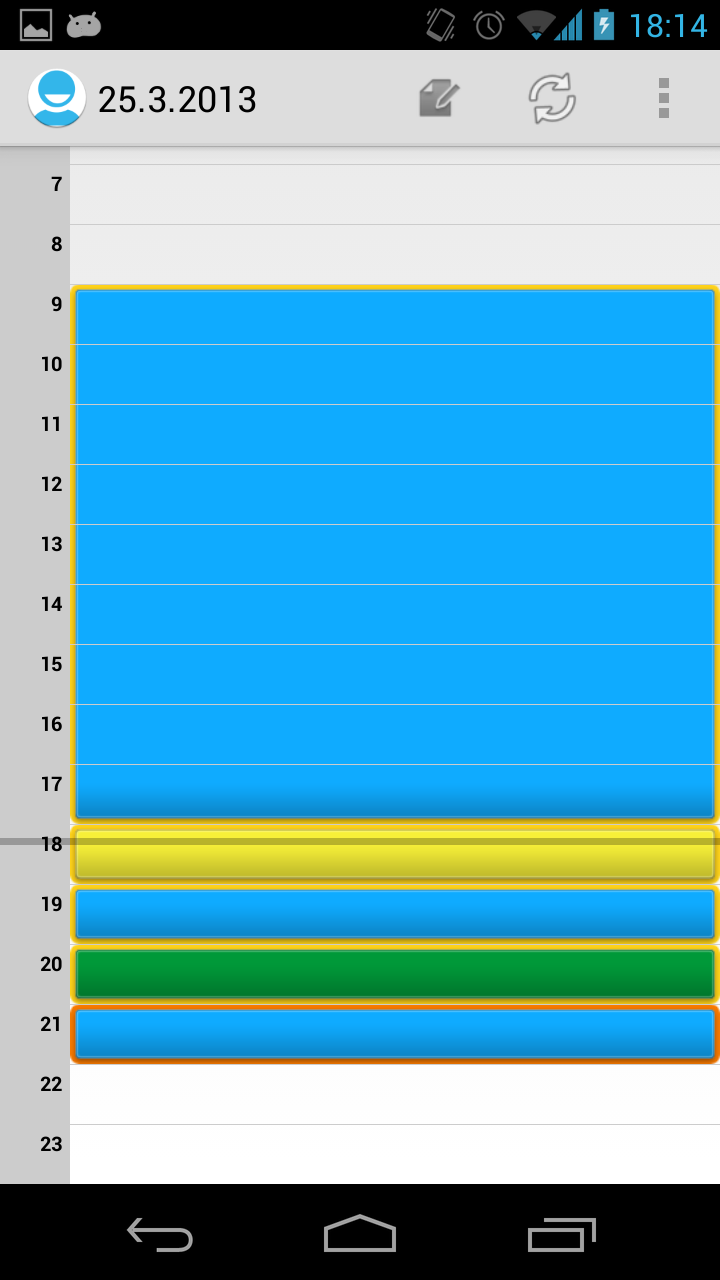
\includegraphics[scale=0.3]{scr/time_doch.png}
  \label{}
\end{figure}

\begin{figure}[H]
  \centering
  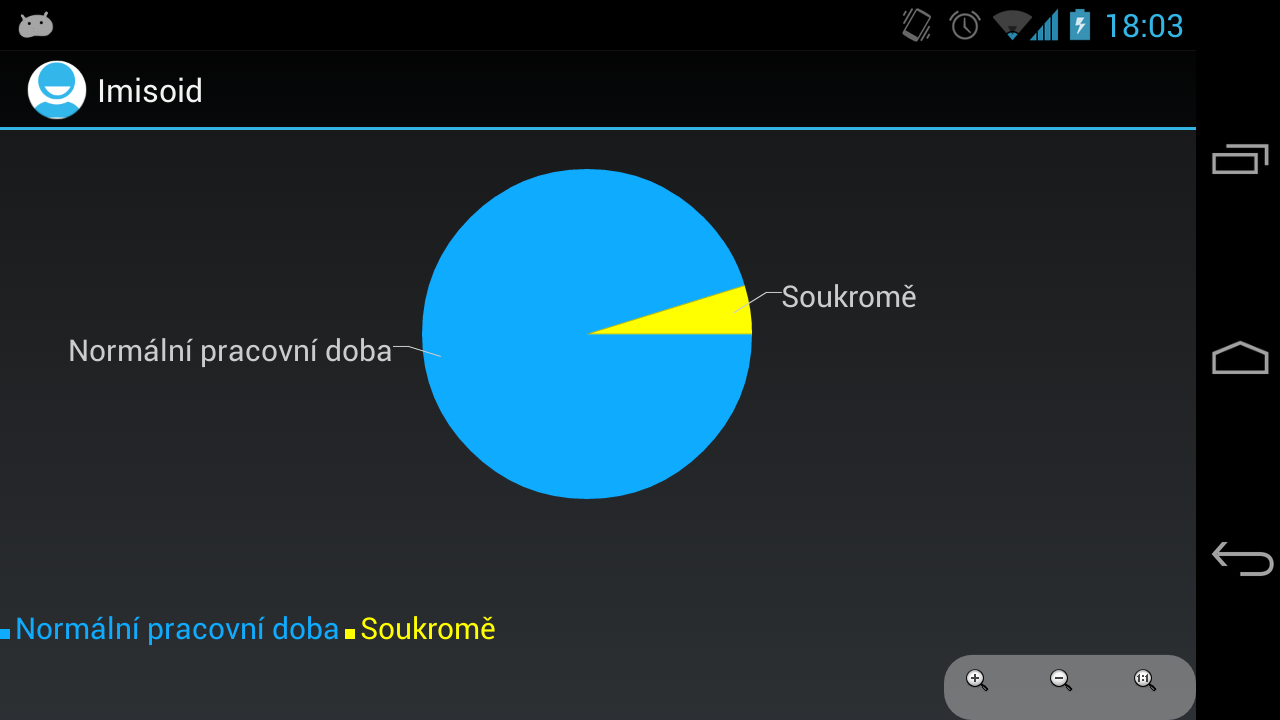
\includegraphics[scale=0.3]{scr/graf_doch.png}
  \label{}
\end{figure}

\begin{figure}[H]
  \centering
  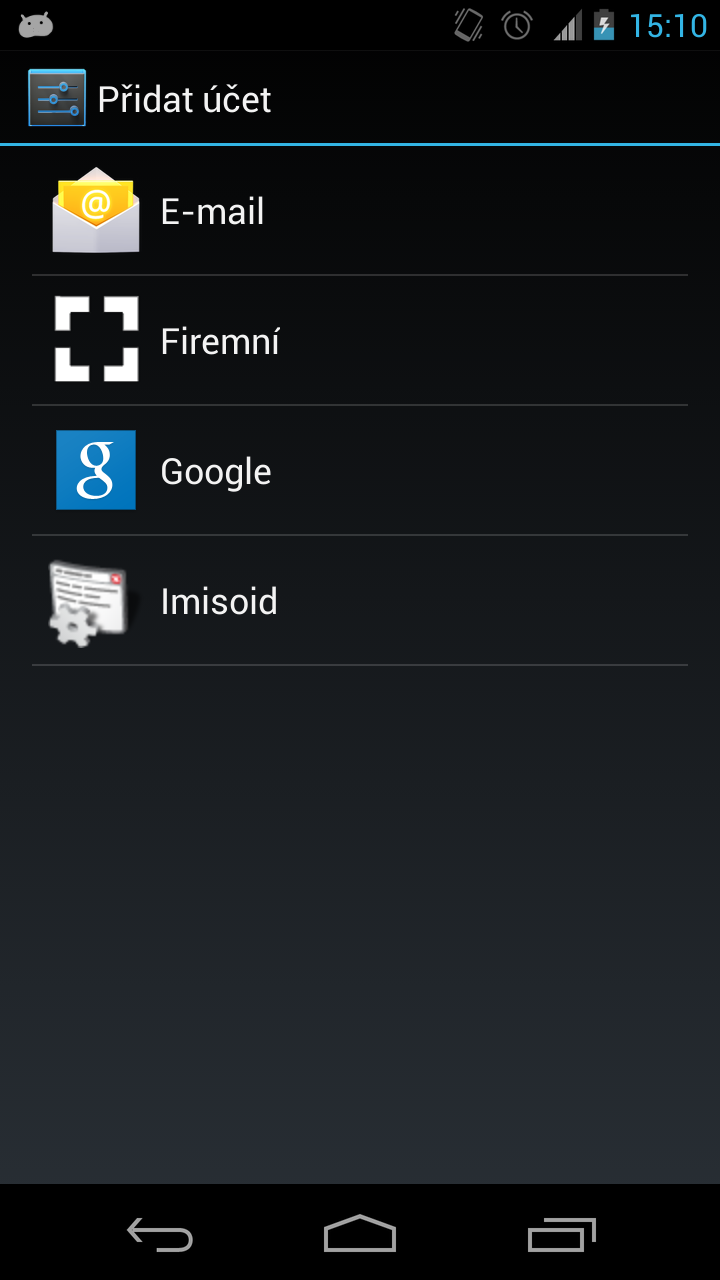
\includegraphics[scale=0.3]{scr/ucet.png}
  \label{}
\end{figure}

\begin{figure}[H]
  \centering
  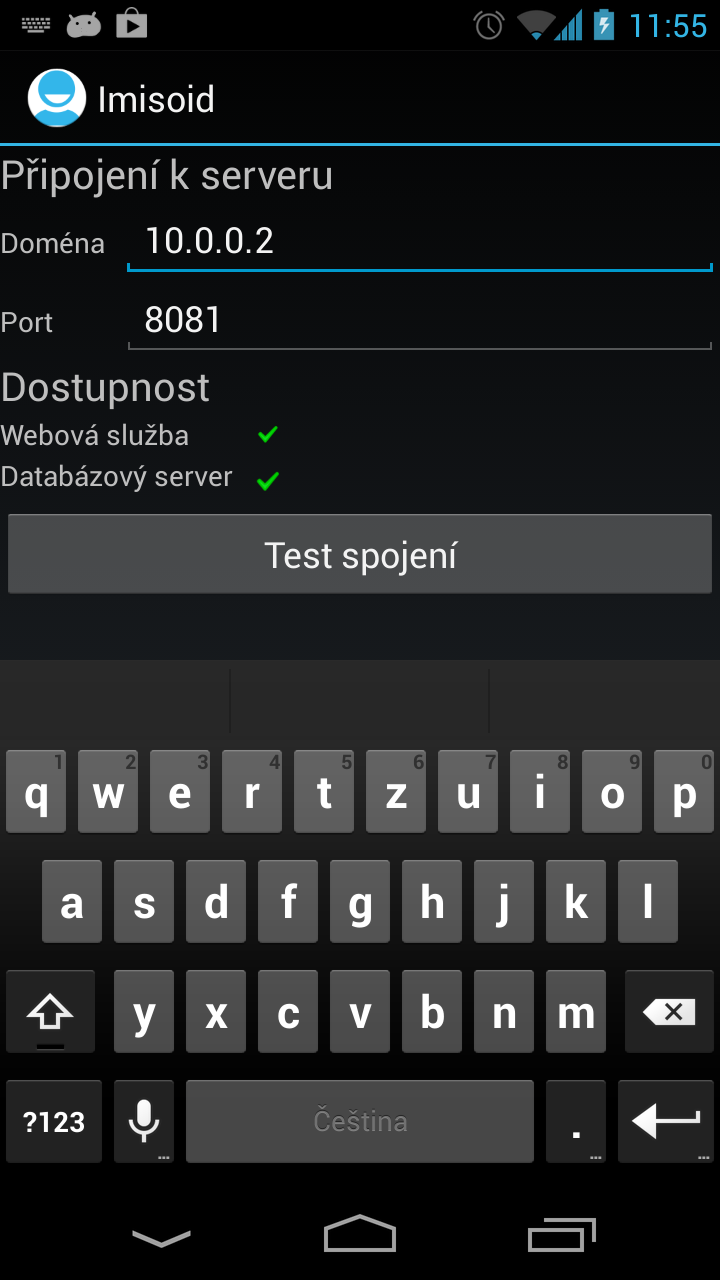
\includegraphics[scale=0.3]{scr/network.png}
  \label{}
\end{figure}

\chapter{Manifest?}

\end{document}
